% Manuscrito generado desde el simulador "Dos mundos que aprenden" (mundos.html).
% Compilar con: latexmk -pdf manuscrito.tex   (las tablas, figuras y macros se generan con: python analisis.py)
\documentclass[11pt,a4paper]{article}
\usepackage[utf8]{inputenc}
\usepackage[T1]{fontenc}
\usepackage[spanish,es-tabla]{babel}
\usepackage{lmodern}
\usepackage[margin=2.5cm]{geometry}
\usepackage{amsmath,amssymb}
\usepackage{booktabs}
\usepackage{graphicx}
\usepackage{caption}
\usepackage{natbib}
\usepackage{microtype}
\usepackage[hidelinks]{hyperref}
\captionsetup{font=small,labelfont=bf}
\setlength{\parskip}{3pt}
\newcommand{\pobAnarq}{365}
\newcommand{\pobAnarqIC}{38}
\newcommand{\prodAnarq}{125}
\newcommand{\prodAnarqIC}{13}
\newcommand{\giniAnarq}{0,40}
\newcommand{\giniAnarqIC}{0,01}
\newcommand{\ataqAnarq}{46,1}
\newcommand{\ataqAnarqIC}{5,2}
\newcommand{\cultivosAnarq}{14}
\newcommand{\cultivosAnarqIC}{3}
\newcommand{\hambrientosAnarq}{2}
\newcommand{\hambrientosAnarqIC}{0}
\newcommand{\prodPcAnarq}{0,34}
\newcommand{\prodPcAnarqIC}{0,01}
\newcommand{\esperanzaAnarq}{51,9}
\newcommand{\esperanzaAnarqIC}{1,4}
\newcommand{\mayorCiudadAnarq}{30}
\newcommand{\mayorCiudadAnarqIC}{11}
\newcommand{\ahorroAnarq}{5,4}
\newcommand{\ahorroAnarqIC}{0,2}
\newcommand{\extAnarq}{0}
\newcommand{\pobAncap}{324}
\newcommand{\pobAncapIC}{33}
\newcommand{\prodAncap}{112}
\newcommand{\prodAncapIC}{12}
\newcommand{\giniAncap}{0,36}
\newcommand{\giniAncapIC}{0,02}
\newcommand{\ataqAncap}{36,9}
\newcommand{\ataqAncapIC}{5,5}
\newcommand{\cultivosAncap}{21}
\newcommand{\cultivosAncapIC}{3}
\newcommand{\hambrientosAncap}{2}
\newcommand{\hambrientosAncapIC}{0}
\newcommand{\prodPcAncap}{0,35}
\newcommand{\prodPcAncapIC}{0,01}
\newcommand{\esperanzaAncap}{48,5}
\newcommand{\esperanzaAncapIC}{1,4}
\newcommand{\mayorCiudadAncap}{30}
\newcommand{\mayorCiudadAncapIC}{8}
\newcommand{\ahorroAncap}{6,0}
\newcommand{\ahorroAncapIC}{0,2}
\newcommand{\extAncap}{0}
\newcommand{\pobMinimo}{228}
\newcommand{\pobMinimoIC}{45}
\newcommand{\prodMinimo}{75}
\newcommand{\prodMinimoIC}{14}
\newcommand{\giniMinimo}{0,30}
\newcommand{\giniMinimoIC}{0,03}
\newcommand{\ataqMinimo}{13,6}
\newcommand{\ataqMinimoIC}{2,6}
\newcommand{\cultivosMinimo}{27}
\newcommand{\cultivosMinimoIC}{6}
\newcommand{\hambrientosMinimo}{1}
\newcommand{\hambrientosMinimoIC}{0}
\newcommand{\prodPcMinimo}{0,33}
\newcommand{\prodPcMinimoIC}{0,01}
\newcommand{\esperanzaMinimo}{38,6}
\newcommand{\esperanzaMinimoIC}{2,9}
\newcommand{\mayorCiudadMinimo}{16}
\newcommand{\mayorCiudadMinimoIC}{4}
\newcommand{\ahorroMinimo}{6,9}
\newcommand{\ahorroMinimoIC}{0,3}
\newcommand{\extMinimo}{0}
\newcommand{\pobSocdem}{241}
\newcommand{\pobSocdemIC}{89}
\newcommand{\prodSocdem}{90}
\newcommand{\prodSocdemIC}{32}
\newcommand{\giniSocdem}{0,17}
\newcommand{\giniSocdemIC}{0,02}
\newcommand{\ataqSocdem}{14,1}
\newcommand{\ataqSocdemIC}{4,7}
\newcommand{\cultivosSocdem}{57}
\newcommand{\cultivosSocdemIC}{18}
\newcommand{\hambrientosSocdem}{0}
\newcommand{\hambrientosSocdemIC}{0}
\newcommand{\prodPcSocdem}{0,37}
\newcommand{\prodPcSocdemIC}{0,02}
\newcommand{\esperanzaSocdem}{42,5}
\newcommand{\esperanzaSocdemIC}{6,1}
\newcommand{\mayorCiudadSocdem}{18}
\newcommand{\mayorCiudadSocdemIC}{8}
\newcommand{\ahorroSocdem}{6,6}
\newcommand{\ahorroSocdemIC}{0,2}
\newcommand{\extSocdem}{0}
\newcommand{\pobSocial}{29}
\newcommand{\pobSocialIC}{13}
\newcommand{\prodSocial}{11}
\newcommand{\prodSocialIC}{5}
\newcommand{\giniSocial}{0,06}
\newcommand{\giniSocialIC}{0,02}
\newcommand{\ataqSocial}{1,5}
\newcommand{\ataqSocialIC}{1,0}
\newcommand{\cultivosSocial}{13}
\newcommand{\cultivosSocialIC}{7}
\newcommand{\hambrientosSocial}{0}
\newcommand{\hambrientosSocialIC}{0}
\newcommand{\prodPcSocial}{0,38}
\newcommand{\prodPcSocialIC}{0,05}
\newcommand{\esperanzaSocial}{13,7}
\newcommand{\esperanzaSocialIC}{5,0}
\newcommand{\mayorCiudadSocial}{4}
\newcommand{\mayorCiudadSocialIC}{1}
\newcommand{\ahorroSocial}{8,5}
\newcommand{\ahorroSocialIC}{2,1}
\newcommand{\extSocial}{1}
\newcommand{\pobComun}{18}
\newcommand{\pobComunIC}{12}
\newcommand{\prodComun}{6}
\newcommand{\prodComunIC}{4}
\newcommand{\giniComun}{0,00}
\newcommand{\giniComunIC}{0,00}
\newcommand{\ataqComun}{0,7}
\newcommand{\ataqComunIC}{0,6}
\newcommand{\cultivosComun}{8}
\newcommand{\cultivosComunIC}{6}
\newcommand{\hambrientosComun}{0}
\newcommand{\hambrientosComunIC}{0}
\newcommand{\prodPcComun}{0,34}
\newcommand{\prodPcComunIC}{0,11}
\newcommand{\esperanzaComun}{8,3}
\newcommand{\esperanzaComunIC}{4,8}
\newcommand{\mayorCiudadComun}{2}
\newcommand{\mayorCiudadComunIC}{1}
\newcommand{\ahorroComun}{8,6}
\newcommand{\ahorroComunIC}{6,0}
\newcommand{\extComun}{3}
\newcommand{\nReplicas}{10}
\newcommand{\nSistemas}{6}
\newcommand{\pSocdemAncapProd}{p=0{,}167}
\newcommand{\dSocdemAncapProd}{-0,66}
\newcommand{\pComunAncapProd}{p<0{,}001}
\newcommand{\dComunAncapProd}{-8,21}
\newcommand{\pAnarqAncapProd}{p=0{,}116}
\newcommand{\dAnarqAncapProd}{0,74}
\newcommand{\pSocdemAncapGini}{p<0{,}001}
\newcommand{\dSocdemAncapGini}{-8,86}
\newcommand{\pComunAncapGini}{p<0{,}001}
\newcommand{\dComunAncapGini}{-24,06}
\newcommand{\pAnarqAncapGini}{p<0{,}001}
\newcommand{\dAnarqAncapGini}{2,21}
\newcommand{\pSocdemAncapPob}{p=0{,}073}
\newcommand{\dSocdemAncapPob}{-0,88}
\newcommand{\pComunAncapPob}{p<0{,}001}
\newcommand{\dComunAncapPob}{-8,78}
\newcommand{\pAnarqAncapPob}{p=0{,}081}
\newcommand{\dAnarqAncapPob}{0,83}
\newcommand{\pSocdemAncapAtaq}{p<0{,}001}
\newcommand{\dSocdemAncapAtaq}{-3,21}
\newcommand{\pComunAncapAtaq}{p<0{,}001}
\newcommand{\dComunAncapAtaq}{-6,67}
\newcommand{\pAnarqAncapAtaq}{p=0{,}013}
\newcommand{\dAnarqAncapAtaq}{1,23}
\newcommand{\pSocdemAncapCult}{p=0{,}001}
\newcommand{\dSocdemAncapCult}{2,00}
\newcommand{\pComunAncapCult}{p<0{,}001}
\newcommand{\dComunAncapCult}{-2,04}
\newcommand{\pAnarqAncapCult}{p=0{,}001}
\newcommand{\dAnarqAncapCult}{-1,72}
\newcommand{\nComparaciones}{25}
\newcommand{\umbralBonferroni}{0,0020}
\newcommand{\umbralImpuesto}{40\,\%}
\newcommand{\umbralImpuestoPrevio}{20\,\%}
\newcommand{\pobImpCero}{321}
\newcommand{\pobImpUno}{17}
\newcommand{\reservaImpCero}{6,0}
\newcommand{\reservaImpUno}{6,5}
\newcommand{\natImpCero}{1,8}
\newcommand{\natImpUno}{0,6}
\newcommand{\prodPcImpCero}{0,34}
\newcommand{\prodPcImpUno}{0,32}
\newcommand{\nReplicasImp}{8}
\newcommand{\pctSobreDiezCero}{9}
\newcommand{\nReservasCero}{945}
\newcommand{\pctSobreDiezVeinte}{5}
\newcommand{\nReservasVeinte}{643}
\newcommand{\pctSobreDiezTotal}{0}
\newcommand{\nReservasTotal}{47}

\newcommand{\nRepMapas}{6}
\newcommand{\etaPobMapa}{0,84}
\newcommand{\pPobMapa}{p<0{,}001}
\newcommand{\etaPobSistema}{0,91}
\newcommand{\pPobSistema}{p<0{,}001}
\newcommand{\etaPobInter}{0,75}
\newcommand{\pPobInter}{p<0{,}001}
\newcommand{\etaProdMapa}{0,82}
\newcommand{\pProdMapa}{p<0{,}001}
\newcommand{\etaProdSistema}{0,89}
\newcommand{\pProdSistema}{p<0{,}001}
\newcommand{\etaProdInter}{0,72}
\newcommand{\pProdInter}{p<0{,}001}
\newcommand{\etaGiniMapa}{0,05}
\newcommand{\pGiniMapa}{p=0{,}081}
\newcommand{\etaGiniSistema}{0,97}
\newcommand{\pGiniSistema}{p<0{,}001}
\newcommand{\etaGiniInter}{0,08}
\newcommand{\pGiniInter}{p=0{,}902}
\newcommand{\etaAtaqMapa}{0,74}
\newcommand{\pAtaqMapa}{p<0{,}001}
\newcommand{\etaAtaqSistema}{0,91}
\newcommand{\pAtaqSistema}{p<0{,}001}
\newcommand{\etaAtaqInter}{0,66}
\newcommand{\pAtaqInter}{p<0{,}001}
\newcommand{\etaCultivosMapa}{0,60}
\newcommand{\pCultivosMapa}{p<0{,}001}
\newcommand{\etaCultivosSistema}{0,64}
\newcommand{\pCultivosSistema}{p<0{,}001}
\newcommand{\etaCultivosInter}{0,50}
\newcommand{\pCultivosInter}{p<0{,}001}
\newcommand{\glError}{180}
\newcommand{\kendallPob}{0,97}
\newcommand{\spearmanPob}{0,97}
\newcommand{\kendallProd}{0,95}
\newcommand{\spearmanProd}{0,94}
\newcommand{\kendallGini}{1,00}
\newcommand{\spearmanGini}{1,00}
\newcommand{\kendallAtaq}{0,96}
\newcommand{\spearmanAtaq}{0,95}
\newcommand{\kendallCultivos}{0,84}
\newcommand{\spearmanCultivos}{0,81}
\newcommand{\mapasSocdemProdMenor}{4}
\newcommand{\mapasSocdemGiniSig}{6}
\newcommand{\mapasComunSig}{6}
\newcommand{\nMapas}{6}
\newcommand{\mapaMejor}{Muchos charcos}
\newcommand{\mapaPeor}{Costa}
\newcommand{\pobMapaMejor}{292}
\newcommand{\pobMapaPeor}{53}
\newcommand{\rhoFertilPob}{1,00}
\newcommand{\rhoDistPob}{-1,00}
\newcommand{\mapaMasComercio}{Muchos charcos}
\newcommand{\intercambiosMapaMas}{7,5}
\newcommand{\mapaMasCiudades}{Río}
\newcommand{\ciudadesMapaMas}{3,6}
\newcommand{\extComunMapas}{7}
\newcommand{\extSocialMapas}{4}
\newcommand{\corridasPorSistema}{36}
\newcommand{\mapasSocdemPobMayor}{0}
\newcommand{\listaMapasSocdemPobMayor}{ninguno}


\title{Del anarcocapitalismo al comunismo en seis geografías:\\ instituciones, incentivos y colapso demográfico en una sociedad artificial que aprende}
\author{Pedro Jesús Guzmán Ramos\thanks{Docente, Instituto de Educación Superior Tecnológico Público ``Sara Sara'', Ayacucho, Perú. Correo: \texttt{pedroguzman@iestpsarasara.edu.pe}. Autor de correspondencia. ORCID: \href{https://orcid.org/0009-0005-5673-7452}{0009-0005-5673-7452}.}}
\date{Octubre de 2026}

\begin{document}
\maketitle

\begin{abstract}
\noindent Se presenta un modelo basado en agentes en el que la biología (hambre, sed, reproducción, mortalidad por edad) y un conjunto mínimo de instintos son fijos, mientras que las decisiones económicas (recolectar, sembrar, regar, invertir, atacar, comerciar, construir) las toma una red neuronal heredada y mutada, de modo que la conducta económica evoluciona por selección natural dentro de la simulación. Sobre esa base se definen seis sistemas económicos (anarquía primitiva, anarcocapitalismo, capitalismo con Estado mínimo, socialdemocracia, socialismo con planificación parcial y comunismo) como combinaciones explícitas de cuatro reglas institucionales: impuesto y frecuencia de reparto, forma del reparto (por igual o según necesidad), propiedad de los cultivos y facilidad para robar. Con \nReplicas{} réplicas por sistema y 200 años simulados, se comparan población, producción, desigualdad, violencia, agricultura y demografía. Dos resultados destacan. Primero, existe un umbral de redistribución mensual (entre \umbralImpuestoPrevio{} y \umbralImpuesto{}) a partir del cual la población colapsa; el mecanismo es distributivo y demográfico, no de esfuerzo: la producción por persona no cambia, pero el reparto comprime la distribución de reservas hasta que casi ninguna pareja reúne lo que cuesta criar, la natalidad se desploma y la edad media al morir cae porque mueren sobre todo niños. Segundo, la socialdemocracia (propiedad protegida, impuesto alto repartido según necesidad) sostiene una producción algo menor que la del anarcocapitalismo (la diferencia es significativa en \mapasSocdemProdMenor{} de \nMapas{} geografías) con la mitad de desigualdad, menos violencia y el triple de agricultura. Un tercer experimento factorial (seis geografías $\times$ seis sistemas, \nRepMapas{} réplicas por celda) muestra que el orden de los sistemas en población, producción y desigualdad es muy estable entre mapas ($W$ de Kendall de \kendallPob{}, \kendallProd{} y \kendallGini{}), que el colapso con reparto alto ocurre en los \nMapas{} mapas, y que la geografía explica una parte sustancial de la varianza de la población (\etaPobMapa{} de $\eta^2_p$) comparable a la de las instituciones (\etaPobSistema). El modelo reproduce seis regularidades conocidas de la literatura (capacidad de carga, distribución de riqueza sesgada, efecto incentivo, derechos de propiedad, respuesta demográfica y asentamiento junto al agua). El simulador, de código abierto y reproducible por semilla, se publica junto con los datos.

\medskip\noindent\textbf{Palabras clave:} simulación basada en agentes; economía computacional; instituciones; redistribución; derechos de propiedad; neuroevolución; Sugarscape.

\medskip\noindent\textbf{From anarcho-capitalism to communism across six geographies: institutions, incentives and demographic collapse in a learning artificial society.}

\noindent\textbf{Abstract.} We present an agent-based model in which biology (hunger, thirst, reproduction, age-dependent mortality) and a minimal set of instincts are fixed, while economic decisions (gathering, sowing, irrigating, investing, attacking, trading, building) are taken by an inherited, mutating neural network, so that economic behaviour evolves by natural selection inside the simulation. On this basis, six economic systems (primitive anarchy, anarcho-capitalism, minimal-state capitalism, social democracy, partially planned socialism and communism) are defined as explicit combinations of four institutional rules: tax rate and frequency, form of redistribution (equal or need-based), property over crops and ease of theft. With \nReplicas{} replicates per system over 200 simulated years we compare population, output, inequality, violence, agriculture and demography. Two findings stand out. First, there is a monthly redistribution threshold (between \umbralImpuestoPrevio{} and \umbralImpuesto{}) beyond which population collapses, through a distributional and demographic mechanism rather than reduced effort: output per person is unchanged, but redistribution compresses the distribution of reserves until almost no couple gathers what it costs to raise a child, births collapse and mean age at death falls because mostly children die. Second, social democracy (protected property, high need-based redistribution) sustains a somewhat lower output than anarcho-capitalism (the difference is significant in \mapasSocdemProdMenor{} of \nMapas{} geographies) with half the inequality, less violence and three times as much farming. A third, factorial experiment (six geographies $\times$ six systems, \nRepMapas{} replicates per cell) shows that the ranking of systems in population, output and inequality is highly stable across maps (Kendall's $W$ of \kendallPob{}, \kendallProd{} and \kendallGini), that the collapse under high redistribution occurs in all \nMapas{} maps, and that geography explains a share of population variance (\etaPobMapa{} partial $\eta^2$) comparable to that of institutions (\etaPobSistema). The model reproduces six stylised facts from the literature. The open-source, seed-reproducible simulator is released with the data.
\end{abstract}

\section{Introducción}
La economía computacional basada en agentes estudia economías como sistemas de agentes heterogéneos que interactúan localmente y de cuya interacción emergen regularidades agregadas \citep{tesfatsion2006ace}. El programa fundacional de \citet{epstein1996growing} mostró que fenómenos como la distribución sesgada de la riqueza, el comercio con precios emergentes o las migraciones pueden ``cultivarse'' a partir de reglas simples en un paisaje de recursos. Desde entonces, los modelos de este tipo se han usado para explorar cómo las instituciones (propiedad, impuestos, protección) condicionan los resultados agregados \citep{north1990,axelrod1997}.

Una limitación habitual de esos modelos es que la conducta económica de los agentes está programada: el modelador decide cuándo un agente ahorra, comercia o roba. Este trabajo adopta una estrategia distinta. Se fija lo que en los seres humanos es biología (metabolismo, sed, embarazo, mortalidad por edad) y un conjunto mínimo de instintos de supervivencia (beber, asegurar una reserva mínima de comida, buscar pareja y techo), y se deja que la conducta económica la determine una red neuronal cuyos pesos se heredan con mutación y recombinación. Así, lo que cada población ``aprende'' a hacer con sus recursos es el resultado de la selección natural bajo las reglas institucionales que se le imponen \citep{holland1975,stanley2002neat}. Esto permite preguntar no solo qué resultado produce una institución dada una conducta, sino qué conducta selecciona cada institución.

Sobre esa base se definen siete sistemas económicos (anarquía primitiva, anarcocapitalismo, capitalismo con Estado mínimo, socialdemocracia, socialismo con planificación parcial, comunismo y un sistema mixto de referencia) como combinaciones explícitas de cuatro reglas: tasa y frecuencia del impuesto, forma del reparto, propiedad de los cultivos y facilidad para robar. Todo lo demás es idéntico entre sistemas, de modo que las diferencias observadas se atribuyen solo a esas reglas.

Las contribuciones son cuatro. (1) Un modelo en el que la economía se aprende sobre una biología fija, descrito con el protocolo ODD \citep{grimm2020odd} y validado contra seis regularidades conocidas. (2) Una operacionalización explícita de sistemas económicos como conjuntos de reglas comparables. (3) La identificación de un umbral de redistribución a partir del cual la población colapsa, con un mecanismo distributivo y demográfico identificable. (4) Una prueba de robustez geográfica: el experimento institucional se repite en seis geografías distintas para separar lo que depende de las instituciones de lo que depende del territorio. (5) Un simulador abierto, de un solo archivo y reproducible por semilla, con un motor de experimentos con réplicas y estadística integrado.

\section{Descripción del modelo (protocolo ODD)}
Se sigue la estructura del protocolo ODD en su segunda actualización \citep{grimm2020odd}: propósito y patrones; entidades, variables de estado y escalas; proceso y programación; conceptos de diseño; inicialización; datos de entrada; submodelos.

\subsection{Propósito y patrones}
El propósito es estudiar cómo distintas reglas institucionales afectan la producción, la desigualdad, la violencia, la agricultura y la demografía de una población cuya conducta económica evoluciona por selección. Los patrones usados para evaluar la utilidad del modelo son seis regularidades de la literatura (sección~\ref{sec:validacion}): capacidad de carga malthusiana, distribución sesgada de la riqueza, efecto de la redistribución sobre la producción, efecto de los derechos de propiedad, respuesta de la población a la fecundidad y concentración de asentamientos junto al agua.

\subsection{Entidades, variables de estado y escalas}
\paragraph{Espacio y tiempo.} Rejilla de $48\times30$ celdas. Un paso de tiempo es un mes; un año son 12 pasos. Cada celda es tierra (con fertilidad $f\in[0,1]$ y capacidad de comida $1+9f$), pared (intransitable) o agua. Solo puede haber una persona por celda.
\paragraph{Celdas.} Variables: tipo, fertilidad, comida silvestre disponible, cultivo (0 sin cultivo, $(0,1)$ en crecimiento, 1 maduro), riego, meses sin agua, dueño del cultivo, hogar que la ocupa, y dos campos derivados: distancia por caminos transitables al agua más cercana y número de celdas cultivables (fertilidad $\ge 0{,}15$) a $\le 3$ celdas.
\paragraph{Personas.} Variables: posición, sexo, edad, energía (0--100) y sed (0--100), reserva de comida y de agua, nivel de herramienta y de defensa (0--6), habilidad aprendida (0--1), tres genes (fuerza, inteligencia, resistencia; cada uno en $[0{,}3; 2]$ y con suma 3), hogar al que pertenece, estado reproductivo (meses de embarazo, meses de descanso), destino de migración, estado de enfermedad, y un cerebro: una red neuronal $26\to10\to12$ con activación tangente hiperbólica (289 pesos) cuya salida máxima determina la acción del mes.
\paragraph{Hogares.} Una celda con casa y un conjunto de hasta 5 miembros. Un grupo de 5 o más casas a $\le 2$ celdas entre sí se contabiliza como ciudad.

\subsection{Visión general del proceso y programación}
Cada mes, en este orden: (1) las celdas regeneran comida silvestre y los cultivos crecen o se secan; (2) cada persona, en orden aleatorio, envejece, gasta energía y sed, come y bebe de su reserva si lo necesita, avanza su embarazo y, si llega a la edad adulta en un hogar lleno, se independiza; (3) percibe su entorno y ejecuta, por prioridad, un instinto si aplica o, en su defecto, la acción que decide su cerebro; (4) si es mujer adulta con hogar y pareja adyacente, puede concebir; (5) se recauda y reparte el impuesto con la frecuencia fijada; (6) se eliminan los muertos, se transmiten herencias y se registran estadísticas. El orden de las personas se baraja cada mes.

\subsection{Conceptos de diseño}
\paragraph{Emergencia.} Población, producción, desigualdad, precios del agua, ciudades y migraciones emergen de las decisiones individuales; no están programadas.
\paragraph{Adaptación.} La conducta económica se adapta por neuroevolución: los pesos del cerebro se heredan de ambos padres (cada peso de uno u otro al azar) con mutación (8\,\% de los pesos, $\sigma=0{,}4$). No hay función objetivo explícita: la selección actúa a través de la supervivencia y la reproducción.
\paragraph{Aprendizaje individual.} La habilidad de recolección y cosecha aumenta con la práctica y no se hereda.
\paragraph{Sensado.} Cada persona percibe su energía, sed y reservas, la comida de su celda y la mejor a su alcance (radio 1, o 2 si su inteligencia es $\ge 1{,}25$), la cercanía del agua, su herramienta y defensa, la presencia, reserva y defensa del vecino más rico, su fuerza, su habilidad, el estado del cultivo de su celda y si es sembrable, si hay un cultivo seco cerca, si tiene hogar y a qué distancia, la fertilidad de su celda, la tierra cultivable alrededor, si hay un hogar con sitio cerca, si el cultivo de su celda es ajeno y cuánta agua carga el vecino.
\paragraph{Interacción.} Local: concepción, ataque, robo de cosecha, contagio y comercio ocurren entre celdas adyacentes; el impuesto y el reparto son globales.
\paragraph{Estocasticidad.} Mapa, genes y cerebros iniciales, orden de ejecución, mutaciones, resultado de ataques, concepción y mortalidad por edad son aleatorios con un generador con semilla (mulberry32): la misma semilla y configuración reproduce exactamente la misma historia.
\paragraph{Colectivos.} Hogares (unidad de residencia, herencia y crianza) y ciudades (agregado observacional).
\paragraph{Observación.} Cada 5 meses se registran población, producción, ataques, índice de Gini de las reservas \citep{gini1921}, reserva media, cultivos, porcentaje de hambrientos, genes medios, habilidad, herramienta, defensa, edad media al morir, natalidad, hogares, ciudades, adultos sin hogar, intercambios, precio del agua y enfermos.

\subsection{Inicialización}
Mapa con siete manchas gaussianas de fertilidad y un patrón de agua según el tipo de mapa: cuatro oasis (configuración por defecto, usada en los experimentos 1 y 2), un río que serpentea de lado a lado, un gran lago central, dos oasis en extremos opuestos, una costa (mar a lo largo de un borde) o doce charcos pequeños repartidos. Toda agua lleva orilla fértil ($0{,}7\,e^{-d^2/24{,}5}$ sumado a la fertilidad base). 100 personas (mitad de cada sexo) en familias de cuatro con casa, asentadas a entre 3 y 8 celdas del agua, con edades uniformes entre 0 y el 50\,\% de la esperanza de vida, 20 de comida y 10 de agua, genes aleatorios normalizados y pesos del cerebro $\mathcal{N}(0;0{,}5)$.

\subsection{Datos de entrada}
El modelo no usa datos externos.

\subsection{Submodelos}
\paragraph{Biología.} Gasto mensual de energía $2(0{,}5+0{,}25F+0{,}25I)(1{,}5-0{,}5R)$ y de sed $0{,}8(1{,}3-0{,}3R)$, con $F,I,R$ los genes de fuerza, inteligencia y resistencia. Se come de la reserva cuando la energía baja de 60 (1 comida = 10 energía) y se bebe a $\le 2$ celdas del agua o de la reserva cargada. Energía o sed en cero causan la muerte. La reserva de comida se pudre 0{,}5\,\% al mes. Esperanza de vida $E=80$ años: a partir de $0{,}6E$ el riesgo mensual de morir es $0{,}02\,((\text{edad}-0{,}6E)/(0{,}4E))^2$ y la muerte es segura a $E$.
\paragraph{Recursos y agricultura.} La comida silvestre de cada celda de tierra crece cada mes un 3{,}5\,\% de su capacidad. Sembrar cuesta 2 de comida y solo es posible en tierra fértil ($f\ge0{,}15$) sin casa y con agua alcanzable. En la orilla ($\le 2$ celdas del agua) el cultivo se riega solo; más lejos necesita que alguien le lleve agua cargada (un riego dura unos 6 meses; tres meses sin agua lo secan). Crece a razón $f/12$ por mes y, maduro, rinde $20\,(0{,}75+0{,}25I)(1+0{,}3h)$ de comida, con $h$ la habilidad; si nadie lo cosecha en dos años se pudre. Recolectar comida silvestre rinde $(1+0{,}5T)(0{,}75+0{,}25I)(1+0{,}5h)$ por mes, con $T$ el nivel de herramienta.
\paragraph{Instintos (fijos).} Con sed $<40$ camina hacia el agua. Con reserva $<5$ o energía $<45$ asegura comida (recolecta si hay o camina hacia la mejor a $\le 6$ celdas; si un muro lo bloquea, sigue un mapa de distancias que rodea paredes). Sin hogar, se une al que tenga sitio a $\le 1$ celda o camina hacia uno a $\le 6$; si no hay, emigra a tierra nueva a $\ge 8$ celdas (elegida por tierra cultivable, cercanía del agua y pocas casas) y funda allí su hogar; si no encuentra destino, construye donde está al reunir 5 de comida. A más de 6 celdas de su hogar tiende a volver. Un adulto con reservas se acerca a una persona adulta del otro sexo a $\le 4$ celdas.
\paragraph{Acciones aprendidas.} Ir a comida, ir a agua, recolectar o cosechar, recoger agua, invertir en herramienta (8 de comida, +50\,\% de recolección por nivel), invertir en defensa (6 de comida), atacar, vagar, sembrar, ir a regar, construir casa (5 de comida; la celda deja de producir y de poder cultivarse) y comerciar.
\paragraph{Conflicto.} Atacar al vecino más rico cuesta 6 de energía; la probabilidad de éxito es $eF_a/(eF_a+(0{,}5+D_v)F_v)$, con $e$ la facilidad para robar, $F$ las fuerzas y $D_v$ la defensa de la víctima; el éxito roba el 35\,\% de la comida y del agua de la víctima; el fracaso cuesta 4 de energía más. Con propiedad privada, cosechar un cultivo ajeno cuyo dueño vive se resuelve con la misma fórmula.
\paragraph{Reproducción.} Sexos al 50\,\%. Concibe una mujer adulta (entre 16 y 45 años), con hogar, no embarazada ni en descanso, con energía $\ge 50$, con un hombre adulto en una celda adyacente y 20 de comida entre ambos (el padre aporta hasta la mitad), con probabilidad mensual 0{,}5. Embarazo de 9 meses; el hijo nace en la celda libre más cercana con 10 de comida, entra en el hogar de la madre y hereda genes promediados con mutación gaussiana ($\sigma=0{,}08$) y un cerebro recombinado y mutado. Doce meses de descanso tras el parto. Al cumplir 16 años, quien vive en un hogar con 4 o más miembros se independiza.
\paragraph{Hogares.} Casa de hasta 5 personas. Sin hogar, un adulto gasta 1 de energía extra al mes y no puede criar. Al morir, la reserva pasa por igual a los miembros vivos de su hogar (herencia activada en todos los experimentos). Una casa vacía diez años desaparece.
\paragraph{Comercio.} Con el vecino adyacente que más agua carga, cada uno valora el agua por su tasa marginal de sustitución $\text{TMS}=(\text{comida}+0{,}5)/(\text{agua}+0{,}5)$; si una supera a la otra en más del 10\,\%, quien más valora el agua compra una unidad al precio $\sqrt{\text{TMS}_a\,\text{TMS}_b}$, acotado entre 0{,}2 y 5 \citep[cap.~4]{epstein1996growing}.
\paragraph{Instituciones.} Con la frecuencia fijada se recauda una fracción (el impuesto) de la reserva de comida de cada persona y se reparte por igual o según necesidad (primero se lleva a 8 de reserva a quienes tienen menos, empezando por los más pobres; el resto por igual). La propiedad privada de cultivos y la facilidad para robar se fijan como se indica en la tabla~\ref{tab:sistemas-reglas}. Las enfermedades estaban desactivadas en los experimentos aquí reportados.

\subsection{Aspecto de la simulación}
La figura~\ref{fig:secuencia} muestra un mundo a lo largo del tiempo tal como lo dibuja el simulador: el terreno indica cuánta comida hay (tierra pelada, pasto, arbustos, árboles), las parcelas con surcos son cultivos, las carpas, casas y edificios son hogares de densidad creciente, y cada persona se dibuja según sus genes dominantes y su defensa (campesinos, forzudos, magos, caballeros). En pocas décadas la población se concentra junto al agua, ocupa la tierra fértil con cultivos y forma ciudades; el territorio alejado del agua queda con bosque y sin habitar.

\begin{figure}[htbp]\centering
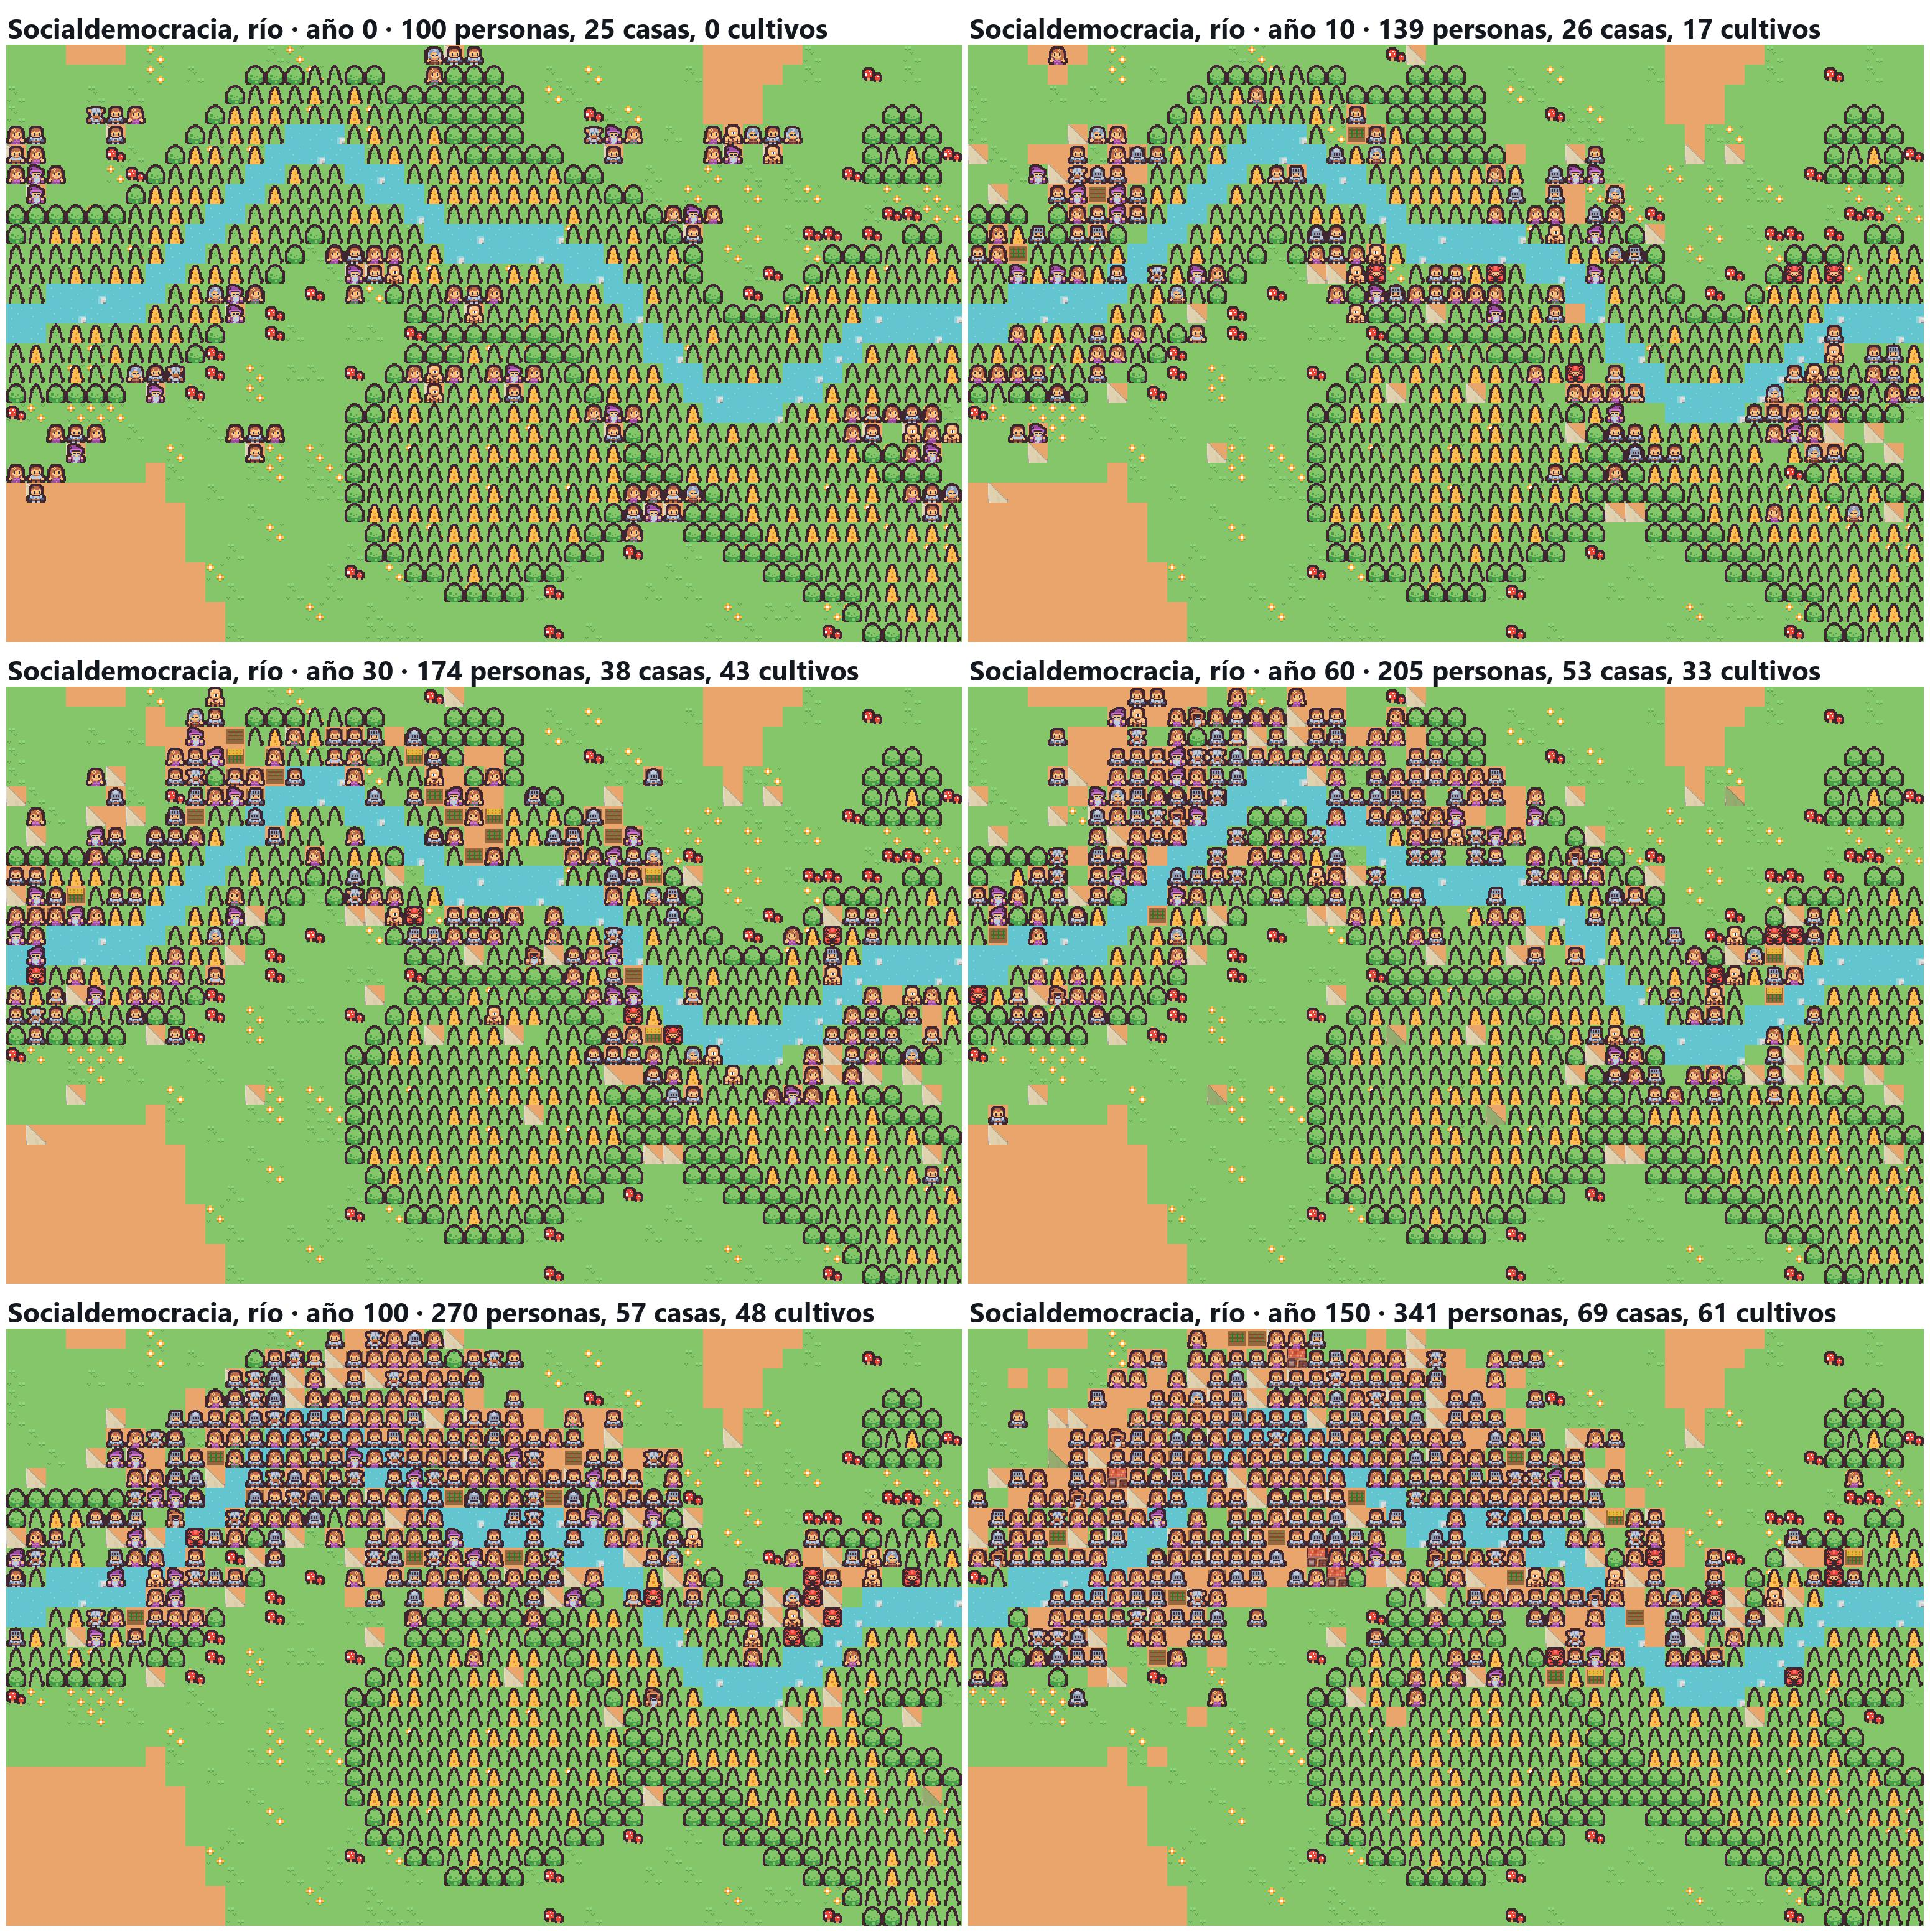
\includegraphics[width=\textwidth]{figuras/mundos_secuencia.pdf}
\caption{Un mundo (socialdemocracia, mapa de río, semilla 2024) en los años 0, 10, 30, 60, 100 y 150. Cada panel indica población, hogares y cultivos.}\label{fig:secuencia}
\end{figure}

\section{Validación por hechos estilizados}\label{sec:validacion}
Antes de usar el modelo para experimentos se comprobó que reproduce regularidades conocidas, el primer nivel de validación recomendado para modelos basados en agentes \citep{windrum2007,fagiolo2019validation}. Cada prueba corre el modelo en dos condiciones con dos semillas durante 80 a 120 años y comprueba una predicción cualitativa (tabla~\ref{tab:validacion}). Las seis se reproducen. Esta validación es cualitativa: indica que el modelo se comporta como los de referencia, no que prediga una economía concreta.

\begin{table}[htbp]\centering\small
\caption{Validación por hechos estilizados (configuración por defecto, 2 semillas por condición, promedio del último 30\,\% de cada corrida).}\label{tab:validacion}
\begin{tabular}{p{3.6cm}p{3.6cm}p{7.6cm}}
\toprule
Regularidad & Referencia & Resultado \\
\midrule
Capacidad de carga & \citet{malthus1798}; \citet{epstein1996growing} & 209 personas con un tercio de la fertilidad frente a 303 con la normal; variación de la población en los últimos 40 años: 3\,\%. \\
Riqueza sesgada & \citet{epstein1996growing} & Gini de reservas 0{,}34; media 6{,}1 mayor que mediana 5{,}4. \\
Redistribución y producción & \citet{okun1975} & Producción total 106 por mes sin reparto frente a 13 con reparto total mensual. \\
Derechos de propiedad & \citet{demsetz1967}; \citet{north1990} & 33{,}4 ataques por mes en anarquía frente a 10{,}8 con Estado; cultivos 18 frente a 28. \\
Fecundidad y población & \citet{verhulst1838} & 201 personas con fecundidad baja frente a 301 con alta. \\
Asentamiento junto al agua & \citet{thunen1826}; \citet{christaller1933} & Viviendas a 3{,}9 celdas del agua frente a 7{,}8 de la tierra en general. \\
\bottomrule
\end{tabular}
\end{table}

\section{Diseño experimental}
\subsection{Sistemas económicos}
Cada sistema es una combinación de las cuatro reglas institucionales (tabla~\ref{tab:sistemas-reglas}). Las demás reglas (biología, instintos, aprendizaje, hogares, migración, comercio, herencia) son idénticas.

\begin{table}[htbp]\centering\small
\caption{Reglas que definen cada sistema económico.}\label{tab:sistemas-reglas}
\resizebox{\textwidth}{!}{\begin{tabular}{lcccc}
\toprule
Sistema & Impuesto (frecuencia) & Reparto & Propiedad de cultivos & Facilidad para robar $e$ \\
\midrule
Anarquía primitiva & 0 & -- & no & 1{,}5 \\
Anarcocapitalismo & 0 & -- & sí & 0{,}7 \\
Capitalismo con Estado mínimo & 10\,\% (12 meses) & por igual & sí & 0{,}2 \\
Socialdemocracia & 35\,\% (3 meses) & según necesidad & sí & 0{,}2 \\
Socialismo (planificación parcial) & 60\,\% (1 mes) & según necesidad & no & 0 \\
Comunismo & 100\,\% (1 mes) & por igual & no & 0 \\
\bottomrule
\end{tabular}}
\end{table}

Se simularon \nReplicas{} réplicas por sistema durante 200 años (2400 meses). La réplica $r$ usa la semilla $2024+7919r$ en todos los sistemas (números aleatorios comunes), de modo que el mapa y la población inicial de la réplica $r$ son idénticos entre sistemas y las comparaciones son pareadas. El valor de cada métrica en una réplica es el promedio de las muestras del último 20\,\% de la duración (los últimos 40 años).

\subsection{Barrido del impuesto}
Para localizar el umbral de colapso se varió el impuesto mensual (0, 20, 40, 60, 80 y 100\,\%) con reparto por igual, cosecha libre y robo posible ($e=0{,}7$), con \nReplicasImp{} réplicas por nivel y 150 años.

\subsection{Geografía por sistema}
Para separar lo que depende de las instituciones de lo que depende del territorio, el experimento 1 se repitió en las seis geografías (tabla~\ref{tab:mapas-geo}) en un diseño factorial completo de 6 mapas $\times$ 6 sistemas con \nRepMapas{} réplicas por celda y 150 años (\corridasPorSistema{} corridas por sistema). Los mapas difieren a la vez en la cantidad de tierra cultivable, en la cantidad de agua y en la distancia media entre la tierra y el agua, de modo que el factor ``mapa'' resume varias propiedades geográficas y no una sola.

\subsection{Análisis estadístico}
Para cada nivel se reporta la media entre réplicas y el intervalo de confianza del 95\,\% (t de Student). En el experimento factorial se ajusta un análisis de varianza de dos factores con interacción (sumas de cuadrados secuenciales: mapa, sistema, mapa $\times$ sistema) y se reporta $\eta^2$ parcial como medida del tamaño del efecto; la estabilidad del orden de los sistemas entre mapas se mide con el coeficiente de concordancia $W$ de Kendall y con la correlación de Spearman media entre los rankings de cada par de mapas. Las comparaciones entre sistemas usan la prueba t de Welch bilateral \citep{welch1947} y el tamaño del efecto $d$ de Cohen \citep{cohen1988}. Con \nComparaciones{} comparaciones frente al anarcocapitalismo, el umbral de Bonferroni equivalente al 5\,\% es $p<\umbralBonferroni$ \citep{dunn1961}.

\section{Resultados}
\subsection{Sistemas económicos}
La tabla~\ref{tab:sistemas} y la figura~\ref{fig:barras} resumen los resultados; la figura~\ref{fig:series} muestra la dinámica temporal y la tabla~\ref{tab:pruebas} las pruebas frente al anarcocapitalismo.

\begin{table}[htbp]\centering\small
\caption{Resultados por sistema económico: media $\pm$ IC 95\,\% entre \nReplicas{} réplicas, promedio de los últimos 40 años de 200. ``ext.'': réplicas extintas.}\label{tab:sistemas}
\resizebox{\textwidth}{!}{\begin{tabular}{lrrrrrrrr}
\toprule
Sistema & Población & Producción (comida/mes) & Gini de reservas & Ataques por mes & Parcelas cultivadas & Hambrientos (\%) & Edad media al morir (años) & Mayor ciudad (hogares) \\
\midrule
Anarquía primitiva & 365 $\pm$ 38 & 125 $\pm$ 13 & 0,40 $\pm$ 0,01 & 46,1 $\pm$ 5,2 & 14 $\pm$ 3 & 2 $\pm$ 0 & 51,9 $\pm$ 1,4 & 30 $\pm$ 11 \\
Anarcocapitalismo & 324 $\pm$ 33 & 112 $\pm$ 12 & 0,36 $\pm$ 0,02 & 36,9 $\pm$ 5,5 & 21 $\pm$ 3 & 2 $\pm$ 0 & 48,5 $\pm$ 1,4 & 30 $\pm$ 8 \\
Capitalismo con Estado mínimo & 228 $\pm$ 45 & 75 $\pm$ 14 & 0,30 $\pm$ 0,03 & 13,6 $\pm$ 2,6 & 27 $\pm$ 6 & 1 $\pm$ 0 & 38,6 $\pm$ 2,9 & 16 $\pm$ 4 \\
Socialdemocracia & 241 $\pm$ 89 & 90 $\pm$ 32 & 0,17 $\pm$ 0,02 & 14,1 $\pm$ 4,7 & 57 $\pm$ 18 & 0 $\pm$ 0 & 42,5 $\pm$ 6,1 & 18 $\pm$ 8 \\
Socialismo (planif. parcial) (1 ext.) & 29 $\pm$ 13 & 11 $\pm$ 5 & 0,06 $\pm$ 0,02 & 1,5 $\pm$ 1,0 & 13 $\pm$ 7 & 0 $\pm$ 0 & 13,7 $\pm$ 5,0 & 4 $\pm$ 1 \\
Comunismo (3 ext.) & 18 $\pm$ 12 & 6 $\pm$ 4 & 0,00 $\pm$ 0,00 & 0,7 $\pm$ 0,6 & 8 $\pm$ 6 & 0 $\pm$ 0 & 8,3 $\pm$ 4,8 & 2 $\pm$ 1 \\
\bottomrule
\end{tabular}
}
\end{table}

\begin{figure}[htbp]\centering
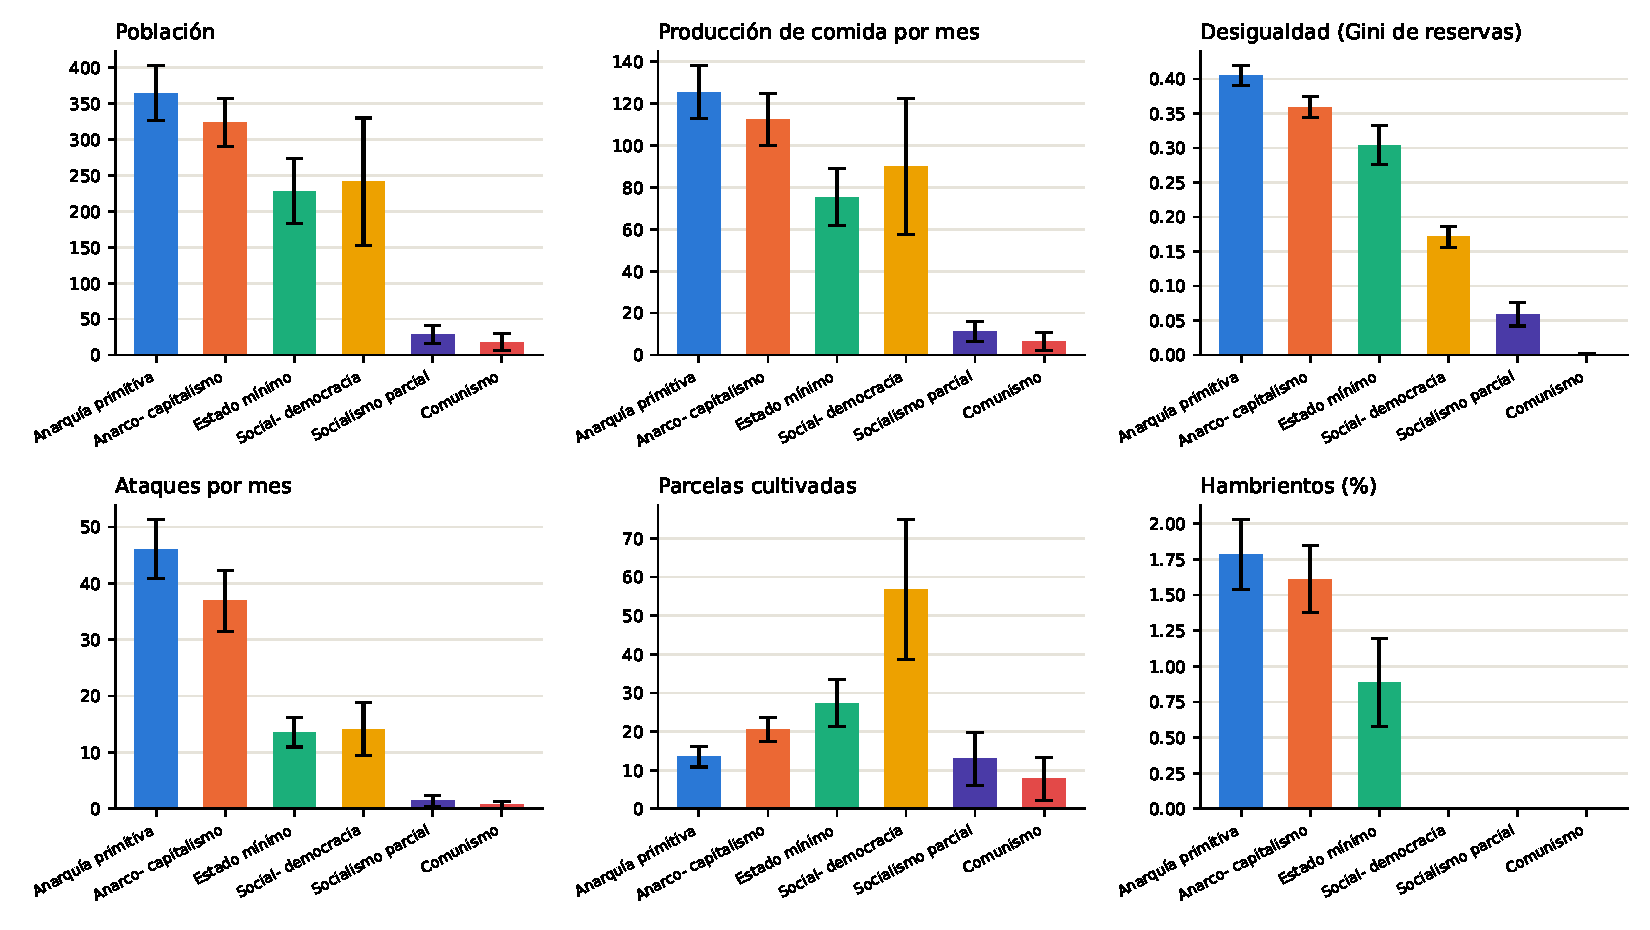
\includegraphics[width=\textwidth]{figuras/sistemas_barras.pdf}
\caption{Seis indicadores por sistema económico (media y IC 95\,\% entre réplicas).}\label{fig:barras}
\end{figure}

\begin{figure}[htbp]\centering
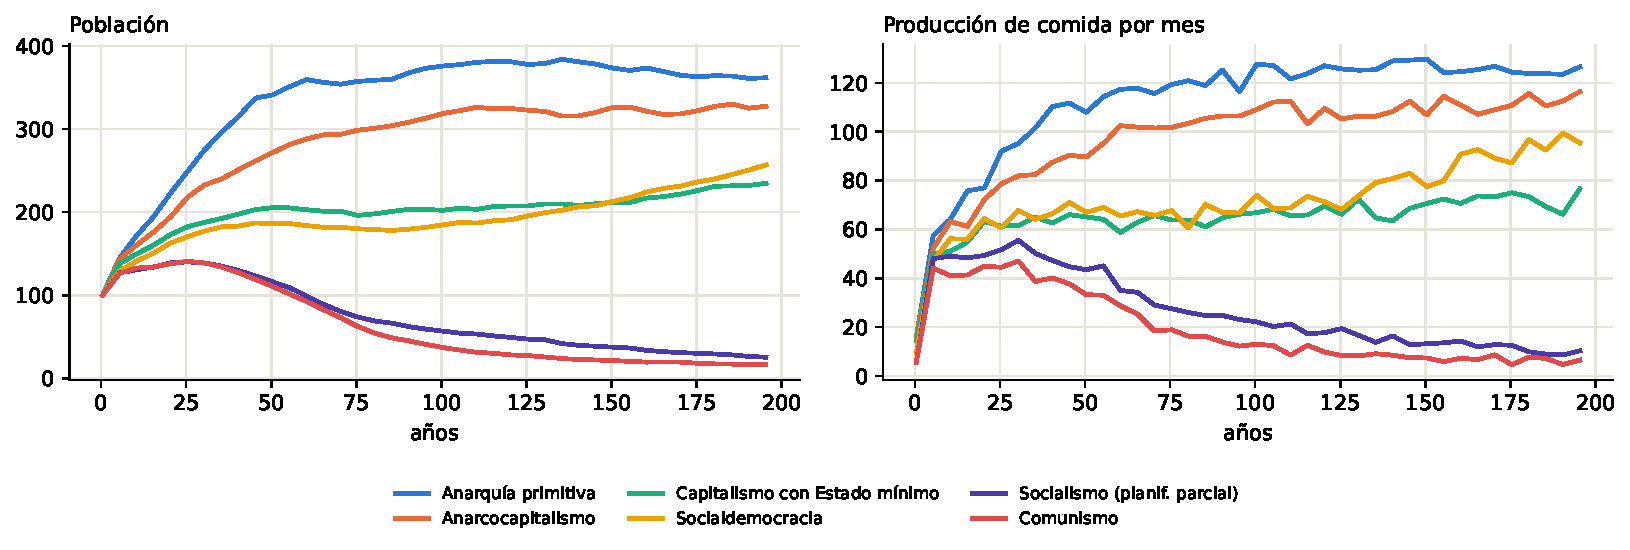
\includegraphics[width=\textwidth]{figuras/series_sistemas.pdf}
\caption{Evolución de la población y de la producción (media de las réplicas) durante 200 años.}\label{fig:series}
\end{figure}

\begin{table}[htbp]\centering\small
\caption{Comparaciones frente al anarcocapitalismo: diferencia de medias, $d$ de Cohen y prueba t de Welch.}\label{tab:pruebas}
\begin{tabular}{llrrr}
\toprule
Métrica & Sistema & Diferencia & $d$ de Cohen & Welch \\
\midrule
Población & Anarquía primitiva & +41 & 0,83 & $p=0{,}081$ \\
 & Capitalismo con Estado mínimo & -96 & -1,73 & $p=0{,}001$ \\
 & Socialdemocracia & -82 & -0,88 & $p=0{,}073$ \\
 & Socialismo (planif. parcial) & -295 & -8,41 & $p<0{,}001$ \\
 & Comunismo & -306 & -8,78 & $p<0{,}001$ \\
\addlinespace
Producción (comida/mes) & Anarquía primitiva & +13 & 0,74 & $p=0{,}116$ \\
 & Capitalismo con Estado mínimo & -37 & -2,05 & $p<0{,}001$ \\
 & Socialdemocracia & -23 & -0,66 & $p=0{,}167$ \\
 & Socialismo (planif. parcial) & -101 & -7,79 & $p<0{,}001$ \\
 & Comunismo & -106 & -8,21 & $p<0{,}001$ \\
\addlinespace
Gini de reservas & Anarquía primitiva & +0,05 & 2,21 & $p<0{,}001$ \\
 & Capitalismo con Estado mínimo & -0,06 & -1,75 & $p=0{,}002$ \\
 & Socialdemocracia & -0,19 & -8,86 & $p<0{,}001$ \\
 & Socialismo (planif. parcial) & -0,30 & -13,52 & $p<0{,}001$ \\
 & Comunismo & -0,36 & -24,06 & $p<0{,}001$ \\
\addlinespace
Ataques por mes & Anarquía primitiva & +9,2 & 1,23 & $p=0{,}013$ \\
 & Capitalismo con Estado mínimo & -23,3 & -3,90 & $p<0{,}001$ \\
 & Socialdemocracia & -22,8 & -3,21 & $p<0{,}001$ \\
 & Socialismo (planif. parcial) & -35,5 & -6,47 & $p<0{,}001$ \\
 & Comunismo & -36,2 & -6,67 & $p<0{,}001$ \\
\addlinespace
Parcelas cultivadas & Anarquía primitiva & -7 & -1,72 & $p=0{,}001$ \\
 & Capitalismo con Estado mínimo & +7 & 1,00 & $p=0{,}043$ \\
 & Socialdemocracia & +36 & 2,00 & $p=0{,}001$ \\
 & Socialismo (planif. parcial) & -8 & -1,04 & $p=0{,}038$ \\
 & Comunismo & -13 & -2,04 & $p<0{,}001$ \\
\addlinespace
\bottomrule
\end{tabular}

\end{table}

\begin{table}[htbp]\centering\small
\caption{Totales acumulados en 200 años (media entre réplicas).}\label{tab:totales}
\resizebox{\textwidth}{!}{\begin{tabular}{lrrrrrr}
\toprule
Sistema & Nacimientos & Muertes por hambre & Ataques & Cosechas robadas & Migraciones & Hogares construidos \\
\midrule
Anarquía primitiva & 1\,445 & 498 & 82\,042 & 0 & 27 & 75 \\
Anarcocapitalismo & 1\,224 & 383 & 65\,211 & 1\,047 & 20 & 70 \\
Capitalismo con Estado mínimo & 861 & 240 & 27\,661 & 815 & 18 & 52 \\
Socialdemocracia & 691 & 0 & 30\,084 & 1\,435 & 19 & 52 \\
Socialismo (planif. parcial) & 160 & 0 & 13\,120 & 0 & 6 & 17 \\
Comunismo & 121 & 0 & 5\,789 & 0 & 5 & 16 \\
\bottomrule
\end{tabular}
}
\end{table}

La figura~\ref{fig:mundos-sistemas} muestra el mismo mundo (mapa de cuatro oasis, semilla 2024) bajo cada sistema al cabo de 150 años. Las diferencias son visibles a simple vista: ciudades densas y campos cultivados en los sistemas sin reparto alto, con muchos caballeros (personas con defensa alta) en los que permiten el robo; y aldeas diminutas con bosques intactos en el socialismo y el comunismo.

\begin{figure}[htbp]\centering
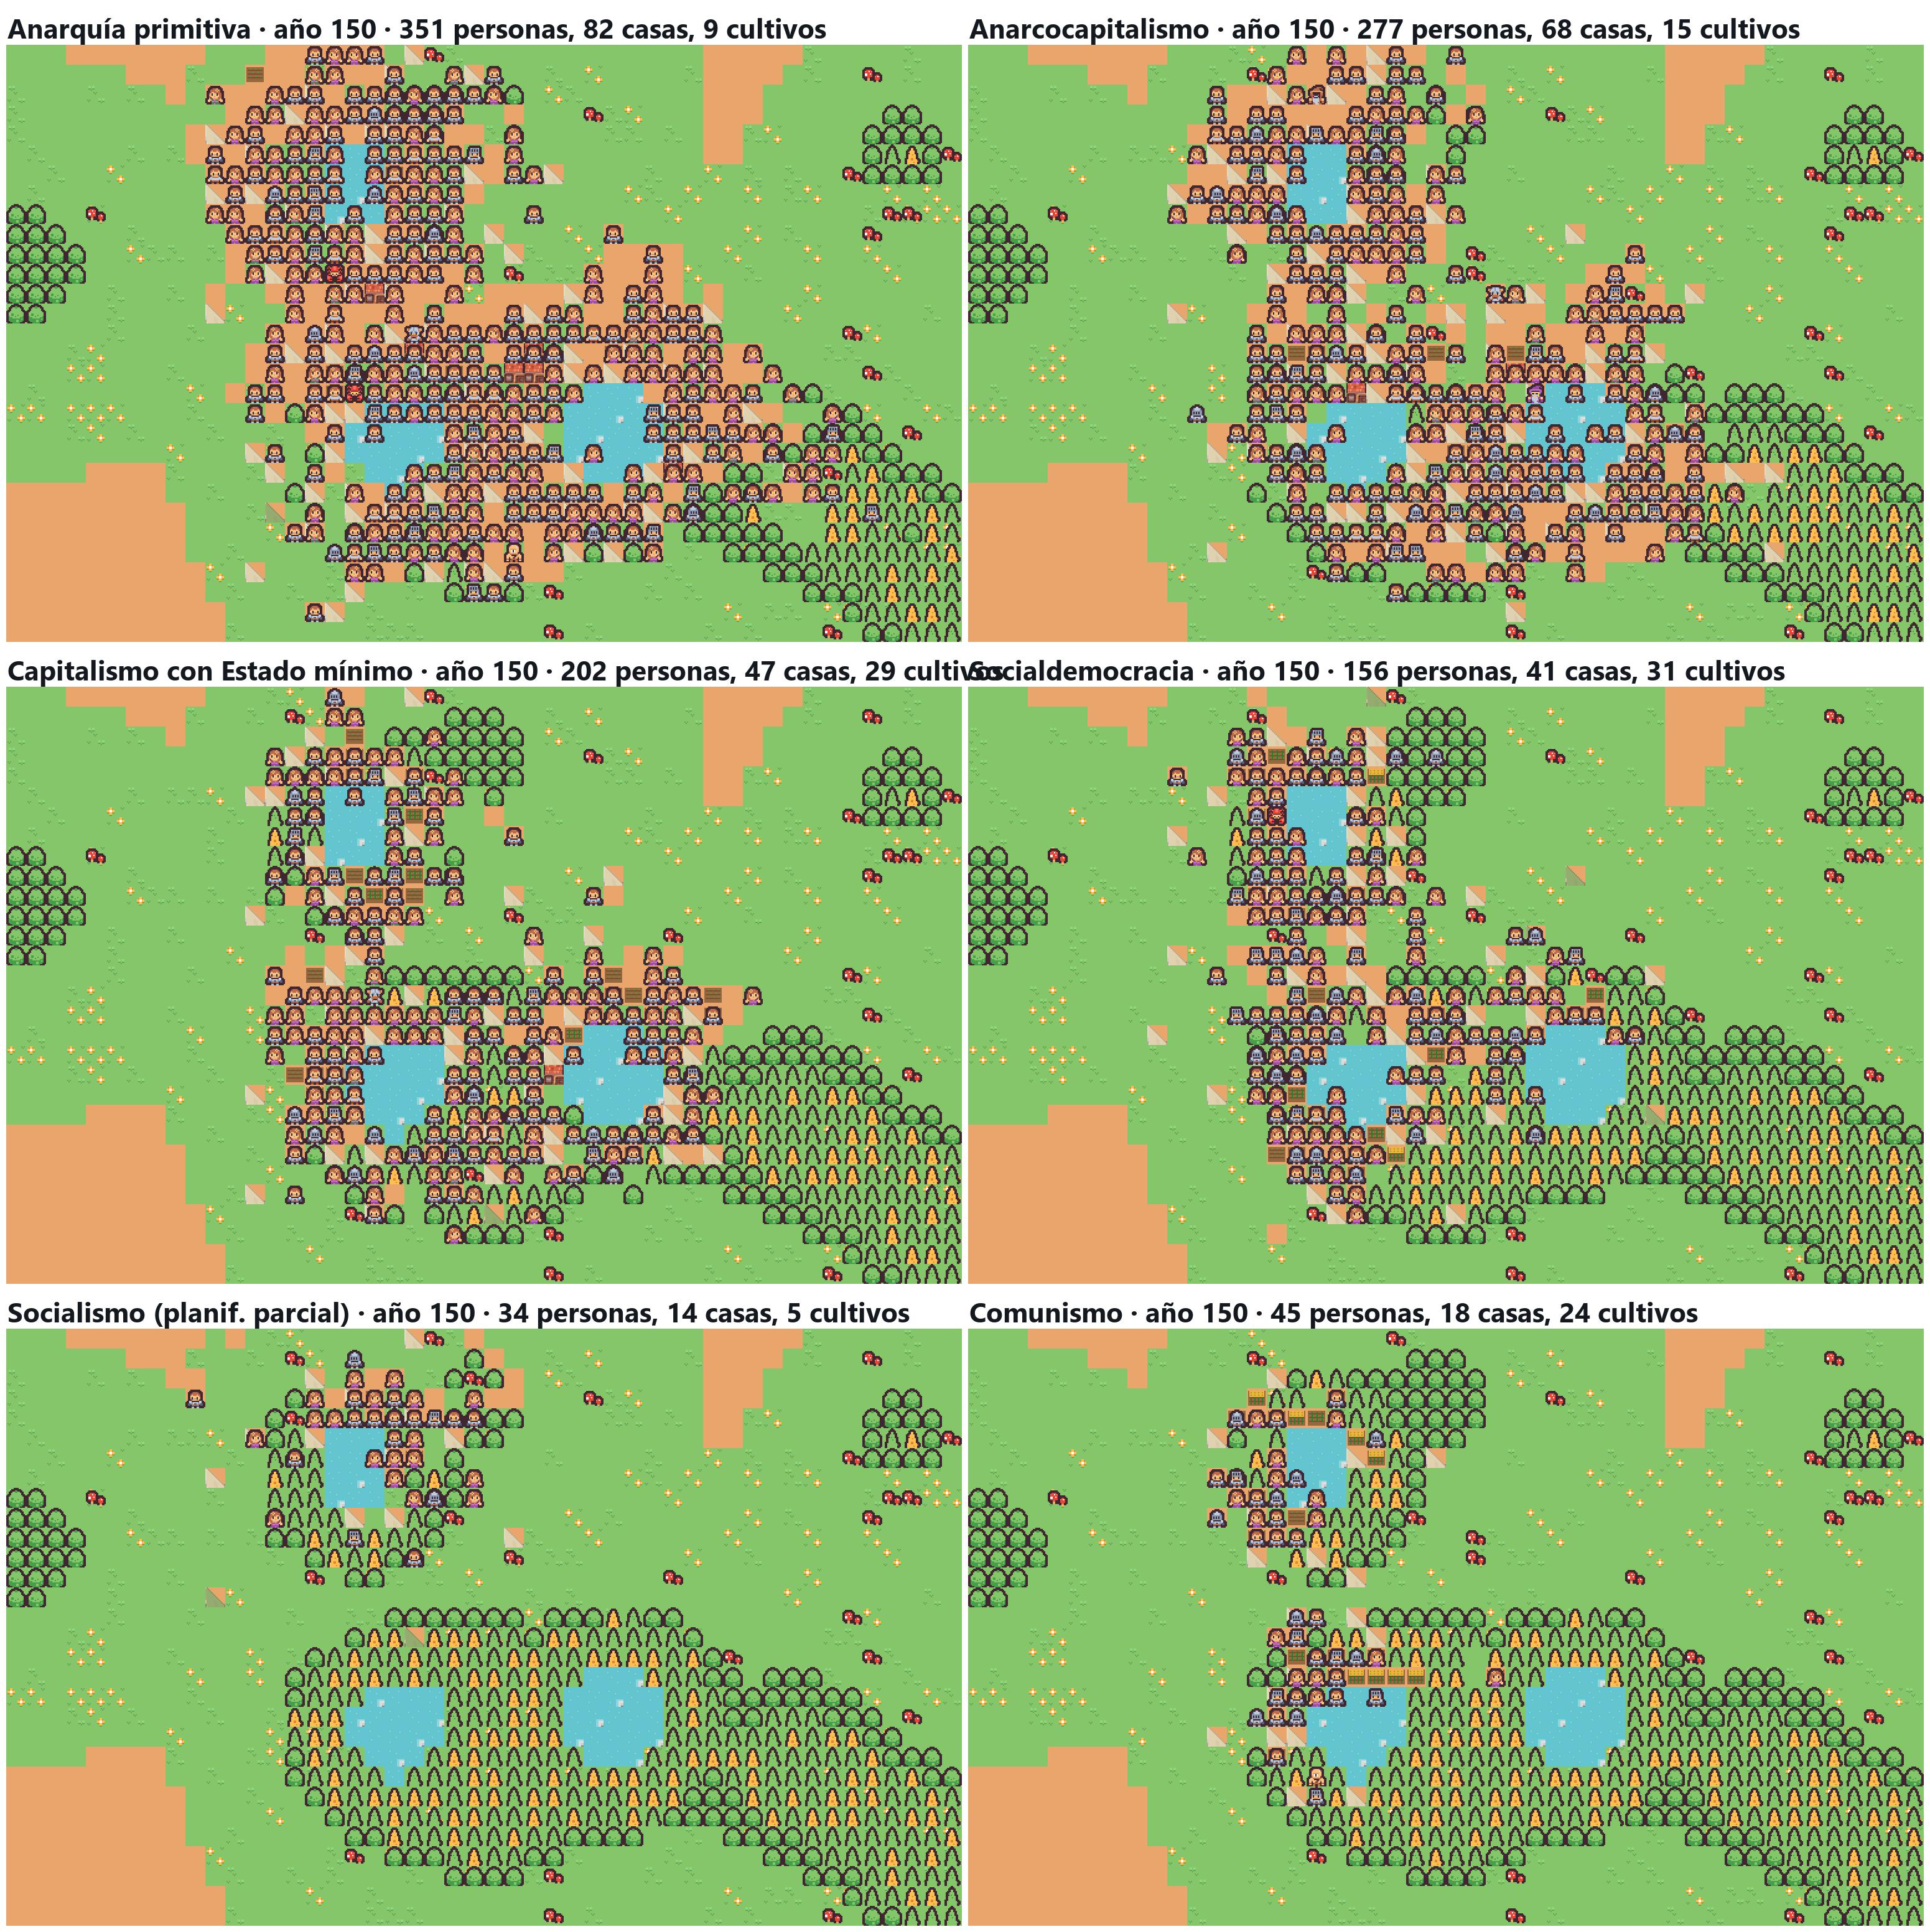
\includegraphics[width=\textwidth]{figuras/mundos_sistemas.pdf}
\caption{El mismo mundo bajo los seis sistemas económicos en el año 150 (mapa de cuatro oasis, semilla 2024, réplica 0 del experimento).}\label{fig:mundos-sistemas}
\end{figure}

Tres grupos de sistemas se distinguen con claridad. Los sistemas sin reparto o con reparto bajo (anarquía primitiva, anarcocapitalismo, capitalismo con Estado mínimo) y la socialdemocracia sostienen poblaciones de entre \pobMinimo{} y \pobAnarq{} personas con producciones de entre \prodMinimo{} y \prodAnarq{} unidades de comida por mes. Los sistemas con reparto mensual alto (socialismo con planificación parcial y comunismo) colapsan a poblaciones de \pobSocial{} y \pobComun{} personas y producciones de \prodSocial{} y \prodComun{} por mes; frente al anarcocapitalismo, la diferencia de población del comunismo tiene $d=\dComunAncapPob$ ($\pComunAncapPob$).

La anarquía primitiva es el sistema con mayor población y producción, pero también el más violento (\ataqAnarq{} ataques por mes frente a \ataqAncap{} en el anarcocapitalismo; $\pAnarqAncapAtaq$) y el más desigual (Gini \giniAnarq{} frente a \giniAncap{}). El anarcocapitalismo, al introducir propiedad privada de los cultivos, convierte parte del conflicto en robos de cosecha (tabla~\ref{tab:totales}) y eleva la inversión en defensa.

La socialdemocracia produce \prodSocdem{} por mes frente a \prodAncap{} del anarcocapitalismo: menos en promedio, pero la diferencia no es significativa con \nReplicas{} réplicas ($\pSocdemAncapProd$; $d=\dSocdemAncapProd$) y su variabilidad entre réplicas es la mayor de todos los sistemas (IC $\pm$\prodSocdemIC). A cambio, su desigualdad es de \giniSocdem{} frente a \giniAncap{} ($\pSocdemAncapGini$; $d=\dSocdemAncapGini$), tiene menos violencia (\ataqSocdem{} ataques por mes frente a \ataqAncap) y casi el triple de agricultura (\cultivosSocdem{} parcelas cultivadas frente a \cultivosAncap{}; $\pSocdemAncapCult$). El capitalismo con Estado mínimo ocupa una posición intermedia: menos violencia que el anarcocapitalismo (\ataqMinimo{} ataques por mes) pero también menos población (\pobMinimo) y producción (\prodMinimo).

\subsection{Umbral de redistribución}
El barrido del impuesto (tabla~\ref{tab:impuesto}, figura~\ref{fig:impuesto}) muestra una caída monótona de la población con el impuesto mensual, de \pobImpCero{} personas sin impuesto a \pobImpUno{} con reparto total; la mitad de la población inicial se pierde entre el \umbralImpuestoPrevio{} y el \umbralImpuesto{}. Dos cantidades no cambian: la producción por persona (\prodPcImpCero{} frente a \prodPcImpUno{} por persona y mes) y la reserva media (\reservaImpCero{} frente a \reservaImpUno). Lo que cambia es la dispersión: el índice de Gini de las reservas pasa de 0{,}34 a 0{,}00. Como criar un hijo exige que la pareja reúna 20 de comida, con una media de 6 solo las parejas de la cola alta de la distribución pueden hacerlo; al comprimir la distribución, el reparto elimina esa cola. La natalidad pasa de \natImpCero{} a \natImpUno{} nacimientos por 100 personas y año. En los sistemas con reparto mensual alto la edad media al morir cae a \esperanzaSocial{} años (socialismo) y \esperanzaComun{} (comunismo), frente a \esperanzaAncap{} en el anarcocapitalismo: la mortalidad se concentra en los niños, que nacen con 10 de comida y no logran reunir más.

La figura~\ref{fig:reservas} hace visible el mecanismo. Como la pareja reúne entre los dos los 20 que cuesta criar, lo relevante es cuántas personas tienen 10 o más: sin impuesto es el \pctSobreDiezCero{}\,\% (la cola alta de la que salen los hijos); con un impuesto mensual del 20\,\% esa fracción cae al \pctSobreDiezVeinte{}\,\%, y con reparto total al \pctSobreDiezTotal{}\,\%, con toda la población concentrada en torno a la media.

\begin{figure}[htbp]\centering
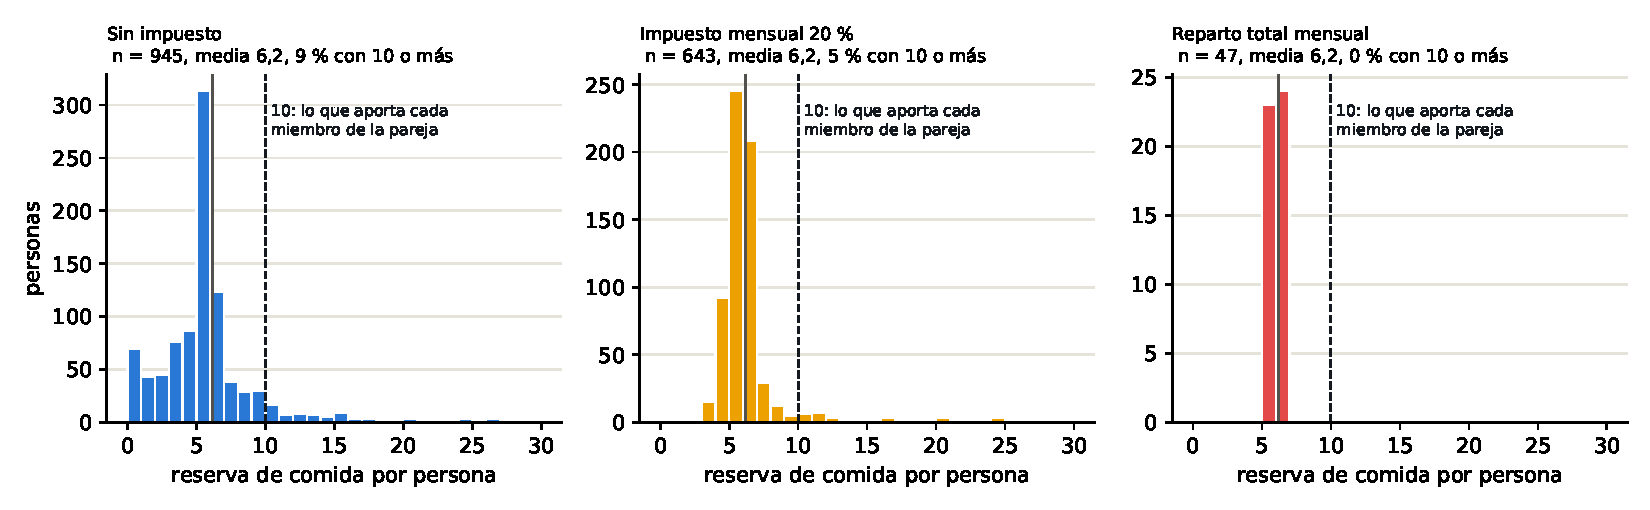
\includegraphics[width=\textwidth]{figuras/reservas.pdf}
\caption{Distribución de la reserva de comida por persona al año 150 (tres réplicas acumuladas) sin impuesto, con impuesto mensual del 20\,\% y con reparto total mensual. La línea discontinua marca 10, la mitad de lo que cuesta criar un hijo (lo que aporta cada miembro de la pareja); la línea continua, la media.}\label{fig:reservas}
\end{figure}

\begin{table}[htbp]\centering\small
\caption{Barrido del impuesto mensual con reparto por igual (media $\pm$ IC 95\,\%, \nReplicasImp{} réplicas, últimos 30 años de 150).}\label{tab:impuesto}
\resizebox{\textwidth}{!}{\begin{tabular}{rrrrrrr}
\toprule
Impuesto mensual & Población & Producción/mes & Producción por persona & Reserva media & Natalidad & Gini \\
\midrule
0\,\% & 321 $\pm$ 31 & 108 $\pm$ 11 & 0,34 $\pm$ 0,01 & 6,0 $\pm$ 0,2 & 1,8 $\pm$ 0,1 & 0,34 $\pm$ 0,02 \\
20\,\% & 215 $\pm$ 45 & 76 $\pm$ 17 & 0,35 $\pm$ 0,01 & 6,2 $\pm$ 0,1 & 1,6 $\pm$ 0,2 & 0,13 $\pm$ 0,01 \\
40\,\% & 137 $\pm$ 50 & 48 $\pm$ 20 & 0,34 $\pm$ 0,02 & 6,2 $\pm$ 0,1 & 1,6 $\pm$ 0,2 & 0,08 $\pm$ 0,00 \\
60\,\% & 66 $\pm$ 34 & 23 $\pm$ 13 & 0,34 $\pm$ 0,02 & 6,2 $\pm$ 0,1 & 1,1 $\pm$ 0,4 & 0,04 $\pm$ 0,00 \\
80\,\% & 23 $\pm$ 11 & 7 $\pm$ 4 & 0,32 $\pm$ 0,05 & 6,3 $\pm$ 0,2 & 0,8 $\pm$ 0,5 & 0,02 $\pm$ 0,00 \\
100\,\% & 17 $\pm$ 4 & 6 $\pm$ 2 & 0,32 $\pm$ 0,05 & 6,5 $\pm$ 0,1 & 0,6 $\pm$ 0,4 & 0,00 $\pm$ 0,00 \\
\bottomrule
\end{tabular}
}
\end{table}

\begin{figure}[htbp]\centering
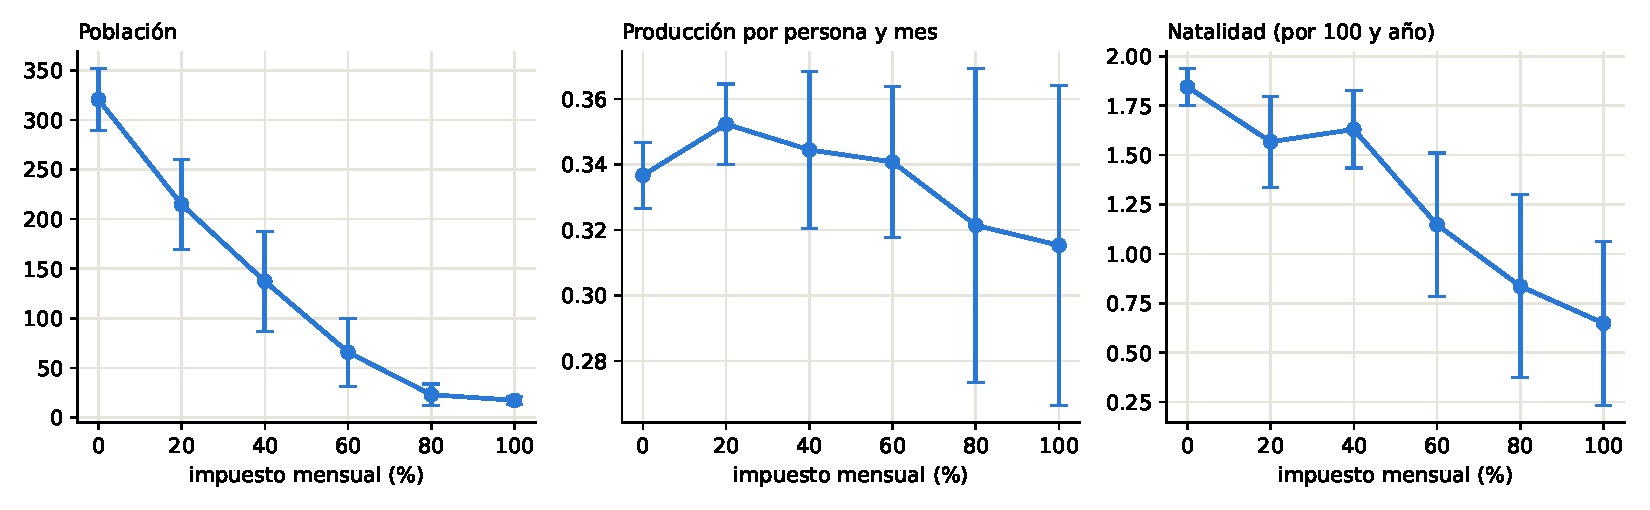
\includegraphics[width=\textwidth]{figuras/impuesto.pdf}
\caption{Población, producción por persona y natalidad en función del impuesto mensual (media y IC 95\,\%).}\label{fig:impuesto}
\end{figure}

\subsection{Robustez geográfica}
Las seis geografías difieren mucho en recursos (tabla~\ref{tab:mapas-geo}): la cantidad de tierra cultivable, la de agua y la distancia media entre ambas. Promediando sobre los sistemas, el mapa más favorable (\mapaMejor) sostiene \pobMapaMejor{} personas y el menos favorable (\mapaPeor) \pobMapaPeor{} (tabla~\ref{tab:mapas-efectos}). Entre los seis mapas, la población correlaciona con la tierra cultivable ($\rho=\rhoFertilPob$) y negativamente con la distancia media al agua ($\rho=\rhoDistPob$). El comercio es más intenso en \mapaMasComercio{} (\intercambiosMapaMas{} intercambios por mes) y el mayor número de ciudades aparece en \mapaMasCiudades{} (\ciudadesMapaMas{} en promedio).

\begin{table}[htbp]\centering\small
\caption{Propiedades geográficas de los seis mapas (promedio de las réplicas).}\label{tab:mapas-geo}
\begin{tabular}{lrrr}
\toprule
Mapa & Celdas de agua & Celdas cultivables & Distancia media al agua \\
\midrule
4 oasis & 64 & 1\,062 & 7,5 \\
Río & 96 & 1\,088 & 5,9 \\
Lago central & 81 & 975 & 9,5 \\
Dos oasis lejanos & 42 & 1\,050 & 8,1 \\
Costa & 90 & 944 & 23,0 \\
Muchos charcos & 37 & 1\,290 & 4,9 \\
\bottomrule
\end{tabular}

\end{table}

\begin{table}[htbp]\centering\small
\caption{Efecto principal del mapa: promedio de los seis sistemas, últimos 30 años de 150.}\label{tab:mapas-efectos}
\resizebox{\textwidth}{!}{\begin{tabular}{lrrrrrrr}
\toprule
Mapa & Población & Producción & Gini & Ataques & Intercambios/mes & Ciudades & Migraciones \\
\midrule
Muchos charcos & 292 & 102 & 0,22 & 23,6 & 7,5 & 3,1 & 22 \\
Río & 262 & 91 & 0,22 & 22,6 & 6,3 & 3,6 & 19 \\
4 oasis & 199 & 68 & 0,22 & 16,6 & 4,8 & 2,6 & 13 \\
Dos oasis lejanos & 122 & 41 & 0,21 & 10,6 & 3,1 & 1,8 & 7 \\
Lago central & 118 & 41 & 0,21 & 10,2 & 3,2 & 1,7 & 6 \\
Costa & 53 & 18 & 0,20 & 5,2 & 1,2 & 0,8 & 1 \\
\bottomrule
\end{tabular}
}
\end{table}

El análisis de varianza (tabla~\ref{tab:anova}) muestra que el sistema económico es la fuente principal de varianza en todas las variables, pero que la geografía explica una parte sustancial de la población ($\eta^2_p=\etaPobMapa$ frente a \etaPobSistema{} del sistema) y que la interacción mapa $\times$ sistema es significativa en población ($\pPobMapa$ para el mapa; interacción $\eta^2_p=\etaPobInter$): el efecto de las instituciones depende en magnitud, aunque no en dirección, del territorio. La excepción es la desigualdad: el mapa no tiene efecto sobre el índice de Gini ($\eta^2_p=\etaGiniMapa$, $\pGiniMapa$) ni interacciona con el sistema, de modo que el reparto de la riqueza queda determinado solo por las instituciones.

\begin{table}[htbp]\centering\small
\caption{Análisis de varianza de dos factores (mapa, sistema, interacción) con sumas de cuadrados secuenciales; \glError{} grados de libertad del error.}\label{tab:anova}
\begin{tabular}{llrrrr}
\toprule
Variable & Fuente & g.l. & $F$ & $p$ & $\eta^2_p$ \\
\midrule
Población & Mapa & 5 & 184,2 & $p<0{,}001$ & 0,84 \\
 & Sistema & 5 & 361,0 & $p<0{,}001$ & 0,91 \\
 & Mapa × sistema & 25 & 21,1 & $p<0{,}001$ & 0,75 \\
\addlinespace
Producción & Mapa & 5 & 168,7 & $p<0{,}001$ & 0,82 \\
 & Sistema & 5 & 303,4 & $p<0{,}001$ & 0,89 \\
 & Mapa × sistema & 25 & 18,5 & $p<0{,}001$ & 0,72 \\
\addlinespace
Gini & Mapa & 5 & 2,0 & $p=0{,}081$ & 0,05 \\
 & Sistema & 5 & 1\,176,6 & $p<0{,}001$ & 0,97 \\
 & Mapa × sistema & 25 & 0,6 & $p=0{,}902$ & 0,08 \\
\addlinespace
Ataques & Mapa & 5 & 104,3 & $p<0{,}001$ & 0,74 \\
 & Sistema & 5 & 362,0 & $p<0{,}001$ & 0,91 \\
 & Mapa × sistema & 25 & 14,3 & $p<0{,}001$ & 0,66 \\
\addlinespace
Cultivos & Mapa & 5 & 53,6 & $p<0{,}001$ & 0,60 \\
 & Sistema & 5 & 63,1 & $p<0{,}001$ & 0,64 \\
 & Mapa × sistema & 25 & 7,3 & $p<0{,}001$ & 0,50 \\
\addlinespace
\bottomrule
\end{tabular}

\end{table}

La dirección se conserva: el orden de los sistemas es muy estable entre mapas (tabla~\ref{tab:concordancia}), con $W$ de Kendall de \kendallPob{} para población, \kendallProd{} para producción y \kendallGini{} para desigualdad. La figura~\ref{fig:heatmap} muestra las medias por celda y la figura~\ref{fig:mapas-lineas} el perfil de cada sistema a lo largo de los mapas (tabla completa en la tabla~\ref{tab:matriz-pob}).

\begin{table}[htbp]\centering\small
\caption{Concordancia del orden de los sistemas entre los seis mapas ($W$ de Kendall y correlación de Spearman media entre pares de mapas). Abreviaturas: Anarq.\ anarquía primitiva, Ancap.\ anarcocapitalismo, E.~mín.\ capitalismo con Estado mínimo, Socdem.\ socialdemocracia, Social.\ socialismo parcial, Comun.\ comunismo.}\label{tab:concordancia}
\begin{tabular}{lrrp{6.2cm}}
\toprule
Variable & $W$ de Kendall & $\rho$ media & Orden de sistemas (de mejor a peor) \\
\midrule
Población & 0,97 & 0,97 & Anarq. $>$ Ancap. $>$ E. mín. $>$ Socdem. $>$ Social. $>$ Comun. \\
Producción & 0,95 & 0,94 & Anarq. $>$ Ancap. $>$ Socdem. $>$ E. mín. $>$ Social. $>$ Comun. \\
Gini (menor = mejor) & 1,00 & 1,00 & Comun. $>$ Social. $>$ Socdem. $>$ E. mín. $>$ Ancap. $>$ Anarq. \\
Ataques (menor = mejor) & 0,96 & 0,95 & Comun. $>$ Social. $>$ E. mín. $>$ Socdem. $>$ Ancap. $>$ Anarq. \\
Cultivos & 0,84 & 0,81 & Socdem. $>$ E. mín. $>$ Ancap. $>$ Anarq. $>$ Comun. $>$ Social. \\
\bottomrule
\end{tabular}

\end{table}

\begin{figure}[htbp]\centering
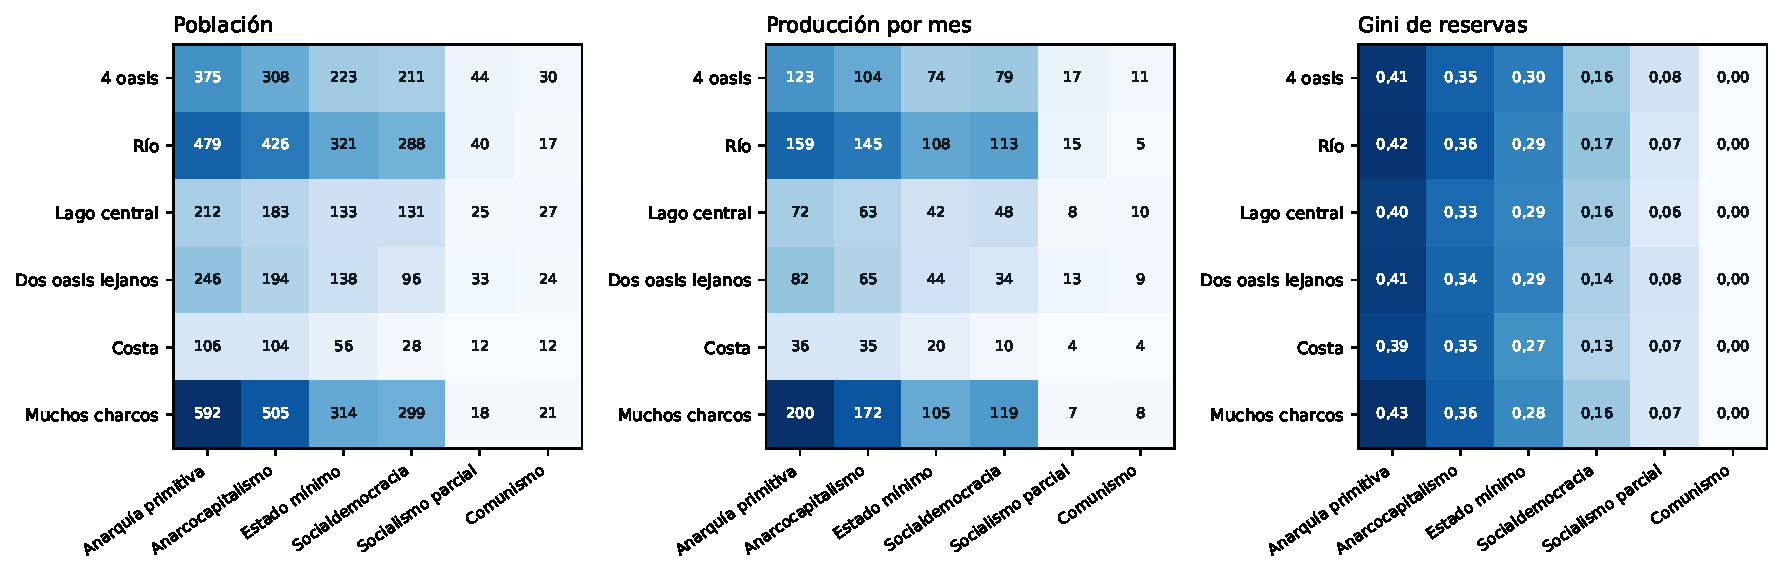
\includegraphics[width=\textwidth]{figuras/mapas_heatmap.pdf}
\caption{Población, producción y desigualdad por mapa y sistema (media de \nRepMapas{} réplicas).}\label{fig:heatmap}
\end{figure}

\begin{figure}[htbp]\centering
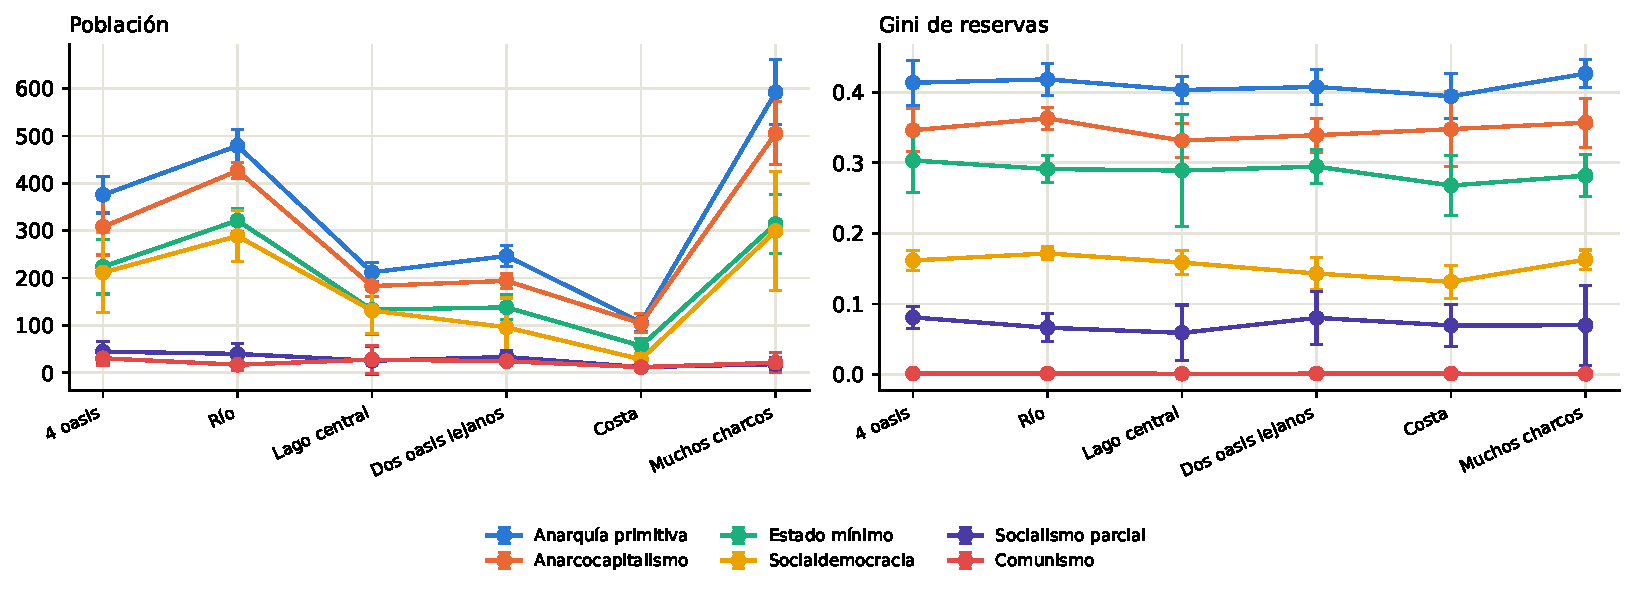
\includegraphics[width=\textwidth]{figuras/mapas_lineas.pdf}
\caption{Perfil de cada sistema a lo largo de las seis geografías (media e IC 95\,\%).}\label{fig:mapas-lineas}
\end{figure}

La figura~\ref{fig:mapas-series} muestra la dinámica completa en cada geografía: la forma de las curvas es la misma en los seis mapas (crecimiento y meseta en los sistemas sin reparto alto, auge breve y declive en socialismo y comunismo), y lo que cambia entre mapas es la altura de la meseta. La figura~\ref{fig:mapas-geo} resume la relación entre geografía y población, con un punto por mapa, y extiende los mapas de calor a la violencia y la agricultura.

\begin{figure}[htbp]\centering
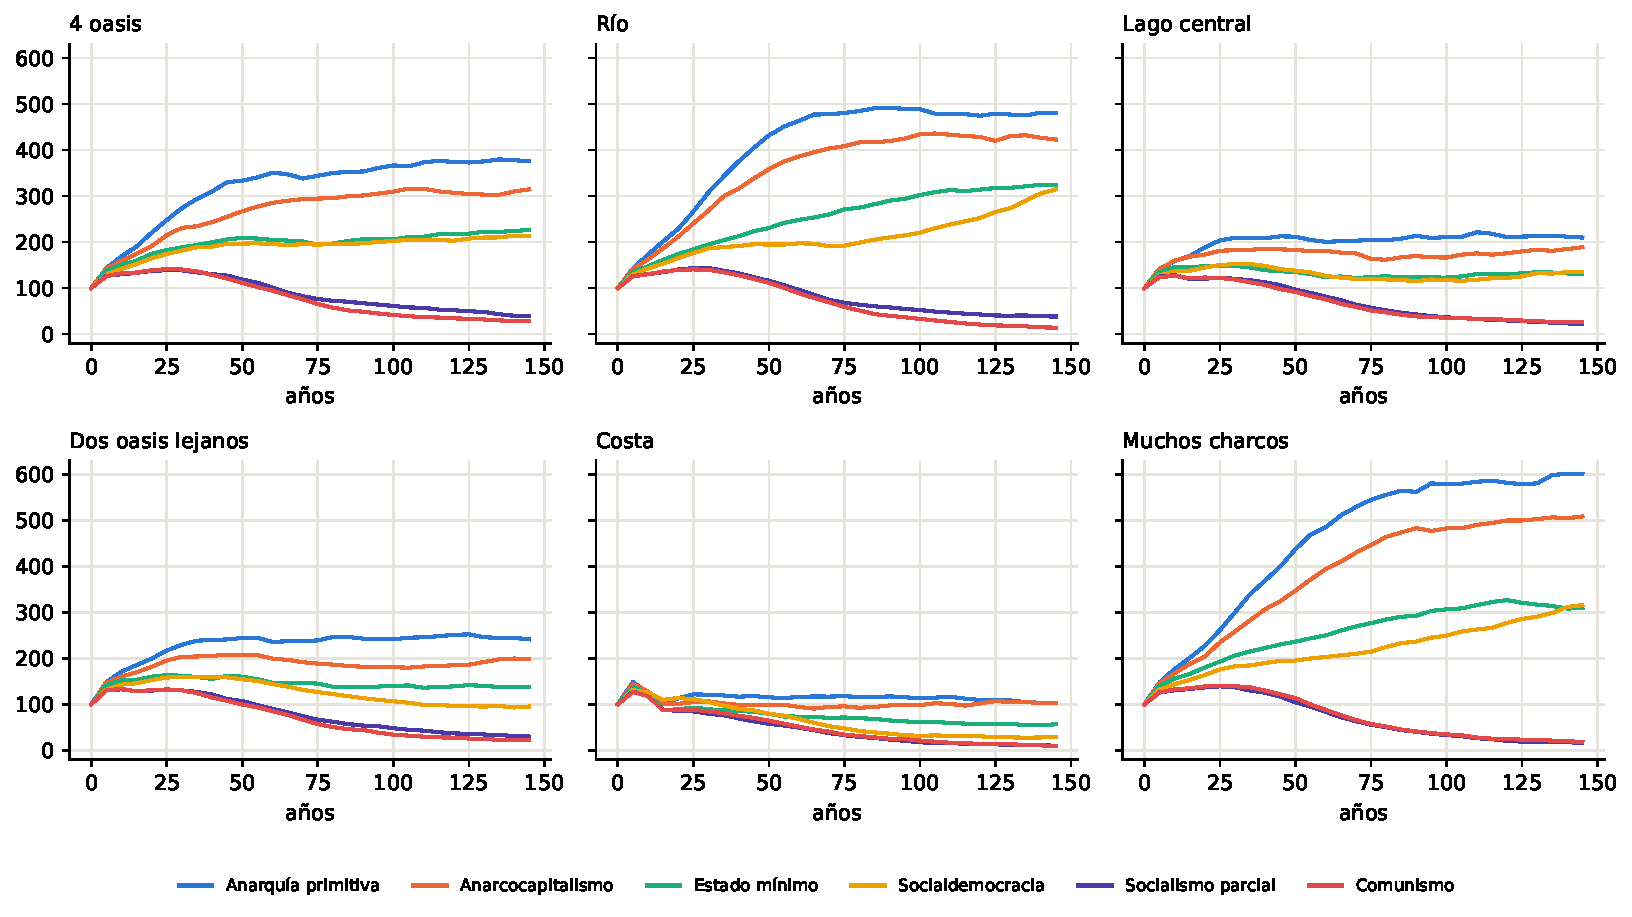
\includegraphics[width=\textwidth]{figuras/mapas_series.pdf}
\caption{Población a lo largo de 150 años en cada geografía (media de \nRepMapas{} réplicas por sistema).}\label{fig:mapas-series}
\end{figure}

\begin{figure}[htbp]\centering
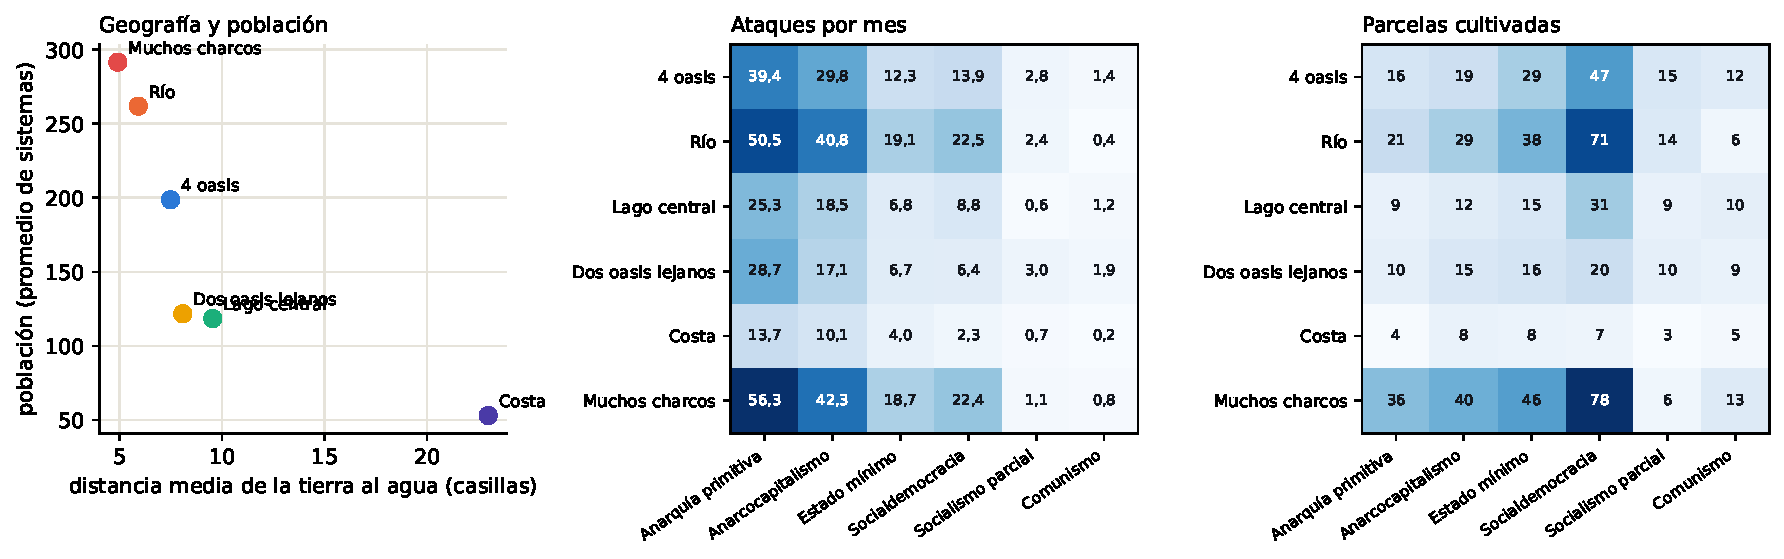
\includegraphics[width=\textwidth]{figuras/mapas_geo.pdf}
\caption{Izquierda: población media (promedio de los seis sistemas) frente a la distancia media de la tierra al agua en cada mapa. Centro y derecha: ataques por mes y parcelas cultivadas por mapa y sistema.}\label{fig:mapas-geo}
\end{figure}

La figura~\ref{fig:mundos-mapas} muestra las seis geografías con el mismo sistema (anarcocapitalismo) en el año 100: se aprecia cómo el poblamiento sigue a la orilla (una franja a lo largo del río, un anillo en torno al lago, una línea estrecha en la costa, un archipiélago de aldeas entre los charcos) y cómo el interior alejado del agua permanece como bosque sin habitar.

\begin{figure}[htbp]\centering
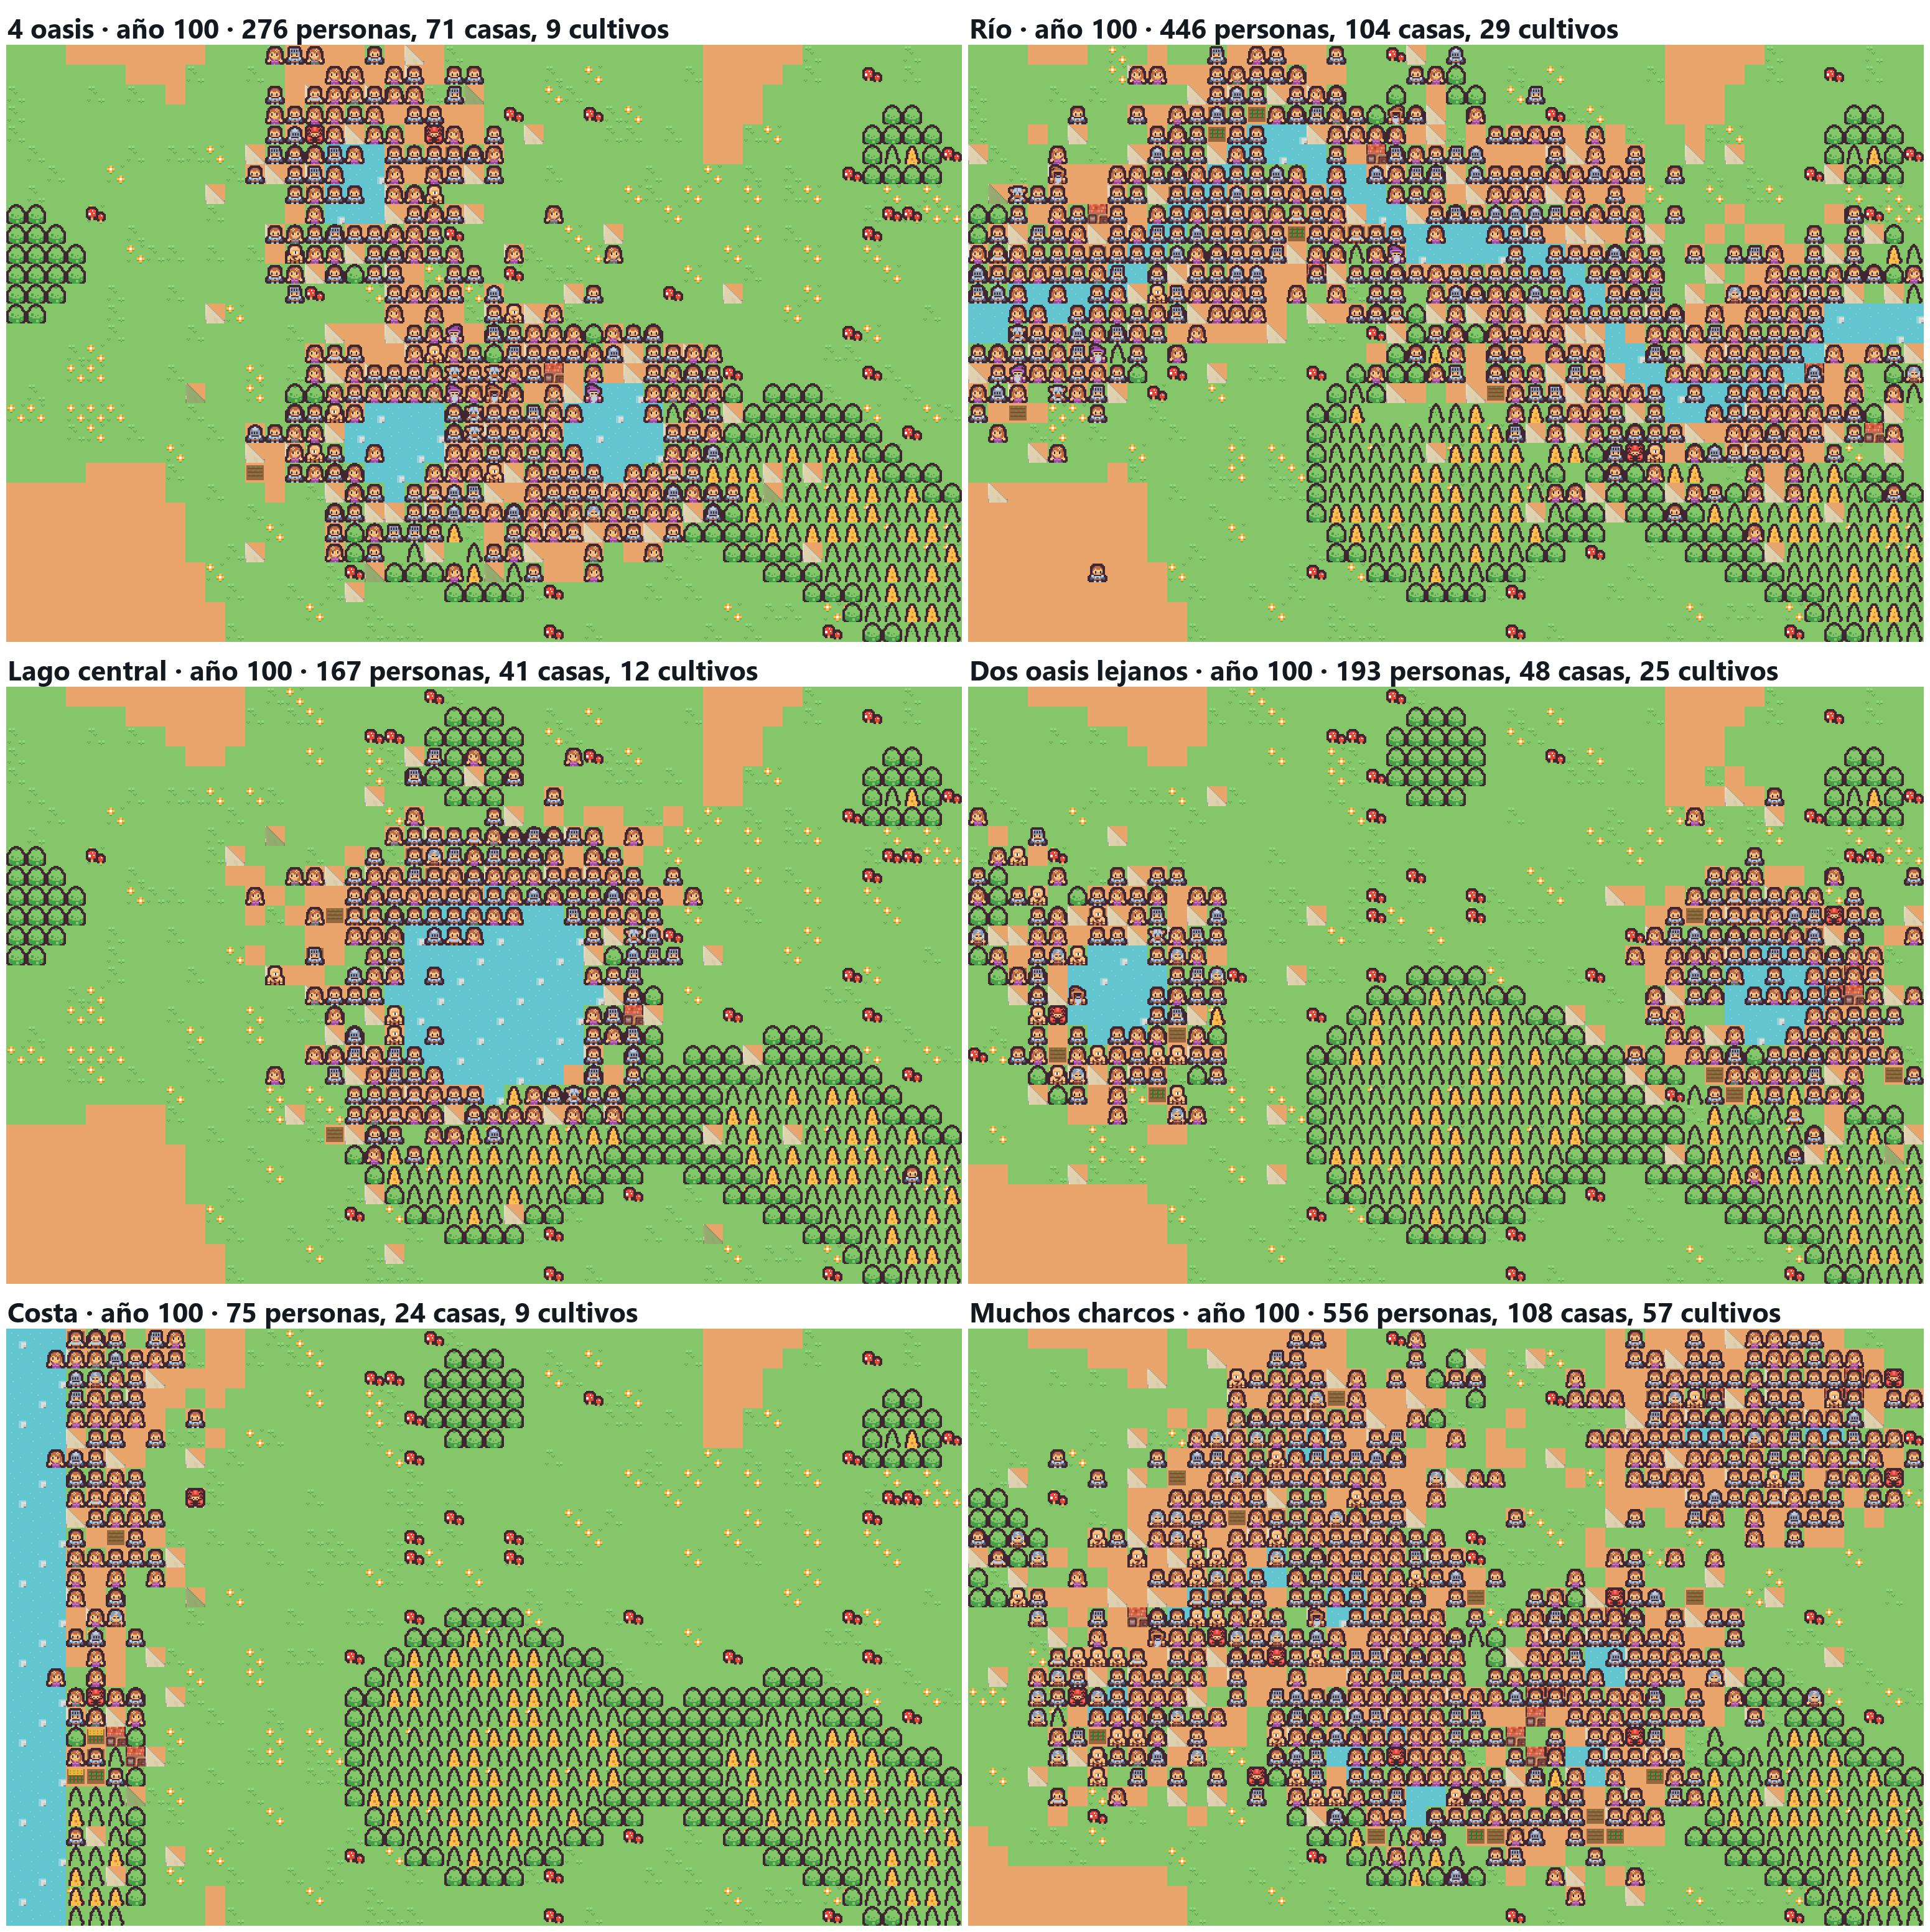
\includegraphics[width=\textwidth]{figuras/mundos_mapas.pdf}
\caption{Las seis geografías bajo el anarcocapitalismo en el año 100 (semilla 2024).}\label{fig:mundos-mapas}
\end{figure}

\begin{table}[htbp]\centering\small
\caption{Población por mapa y sistema (media $\pm$ IC 95\,\%).}\label{tab:matriz-pob}
\resizebox{\textwidth}{!}{\begin{tabular}{lrrrrrr}
\toprule
Mapa & Anarquía primitiva & Anarcocapitalismo & Estado mínimo & Socialdemocracia & Socialismo parcial & Comunismo \\
\midrule
4 oasis & 375 $\pm$ 38 & 308 $\pm$ 59 & 223 $\pm$ 57 & 211 $\pm$ 85 & 44 $\pm$ 22 & 30 $\pm$ 16 \\
Río & 479 $\pm$ 35 & 426 $\pm$ 17 & 321 $\pm$ 24 & 288 $\pm$ 55 & 40 $\pm$ 21 & 17 $\pm$ 13 (2 ext.) \\
Lago central & 212 $\pm$ 20 & 183 $\pm$ 22 & 133 $\pm$ 53 & 131 $\pm$ 48 & 25 $\pm$ 30 (1 ext.) & 27 $\pm$ 30 (1 ext.) \\
Dos oasis lejanos & 246 $\pm$ 22 & 194 $\pm$ 16 & 138 $\pm$ 26 & 96 $\pm$ 62 & 33 $\pm$ 14 & 24 $\pm$ 7 \\
Costa & 106 $\pm$ 19 & 104 $\pm$ 20 & 56 $\pm$ 16 & 28 $\pm$ 13 & 12 $\pm$ 8 (2 ext.) & 12 $\pm$ 8 (2 ext.) \\
Muchos charcos & 592 $\pm$ 69 & 505 $\pm$ 66 & 314 $\pm$ 63 & 299 $\pm$ 126 & 18 $\pm$ 13 (1 ext.) & 21 $\pm$ 21 (2 ext.) \\
\bottomrule
\end{tabular}
}
\end{table}

Los dos contrastes centrales del experimento 1 se sostienen (tabla~\ref{tab:contrastes-mapas}). El colapso del comunismo frente al anarcocapitalismo es significativo en \mapasComunSig{} de los \nMapas{} mapas, y en total \extComunMapas{} de las \corridasPorSistema{} corridas comunistas y \extSocialMapas{} de las socialistas terminaron en extinción. La menor desigualdad de la socialdemocracia es significativa en \mapasSocdemGiniSig{} de \nMapas{} mapas, y su producción es significativamente menor que la del anarcocapitalismo en \mapasSocdemProdMenor{} de \nMapas; en población, la socialdemocracia iguala o supera al anarcocapitalismo en \mapasSocdemPobMayor{} de los \nMapas{} mapas.

\begin{table}[htbp]\centering\small
\caption{Contrastes clave repetidos en cada mapa ($d$ de Cohen y prueba t de Welch, \nRepMapas{} réplicas por sistema y mapa).}\label{tab:contrastes-mapas}
\resizebox{\textwidth}{!}{\begin{tabular}{lrrrrrr}
\toprule
 & \multicolumn{2}{c}{Socdem. vs ancap.: producción} & \multicolumn{2}{c}{Socdem. vs ancap.: Gini} & \multicolumn{2}{c}{Comunismo vs ancap.: población} \\
\cmidrule(lr){2-3}\cmidrule(lr){4-5}\cmidrule(lr){6-7}
Mapa & $d$ & $p$ & $d$ & $p$ & $d$ & $p$ \\
\midrule
4 oasis & -1,07 & $p=0{,}099$ & -8,23 & $p<0{,}001$ & -6,70 & $p<0{,}001$ \\
Río & -2,75 & $p=0{,}003$ & -15,58 & $p<0{,}001$ & -29,03 & $p<0{,}001$ \\
Lago central & -1,05 & $p=0{,}107$ & -8,84 & $p<0{,}001$ & -6,26 & $p<0{,}001$ \\
Dos oasis lejanos & -1,79 & $p=0{,}023$ & -8,76 & $p<0{,}001$ & -14,16 & $p<0{,}001$ \\
Costa & -4,30 & $p<0{,}001$ & -5,52 & $p<0{,}001$ & -6,42 & $p<0{,}001$ \\
Muchos charcos & -1,41 & $p=0{,}046$ & -7,70 & $p<0{,}001$ & -10,29 & $p<0{,}001$ \\
\bottomrule
\end{tabular}
}
\end{table}

\section{Discusión}
\paragraph{Geografía e instituciones.} El experimento factorial permite una afirmación que el experimento 1 por sí solo no permitía: las conclusiones institucionales no son un artefacto de un mapa. El orden de los sistemas se mantiene en seis geografías con cantidades y disposiciones de agua y tierra muy distintas, y el colapso bajo reparto alto ocurre en todas. Al mismo tiempo, la geografía no es un detalle: explica una fracción de la varianza de la población comparable a la de las instituciones y modula el tamaño de los efectos institucionales. Lo que importa del territorio no es cuánta agua hay sino cómo está repartida: los mapas con agua dispersa (muchos charcos, río), donde casi toda la tierra cultivable queda cerca de alguna orilla, sostienen las mayores poblaciones y el mayor comercio; los mapas con el agua concentrada en un solo lugar (lago central, costa) son los peores, aunque la costa tenga la mayor cantidad de agua, porque la mayor parte de la tierra queda lejos de ella y el riego a mano no compensa la distancia. La población entre mapas sigue de forma casi perfecta la distancia media entre la tierra y el agua. En cambio, la desigualdad no depende del mapa en absoluto ($\eta^2_p=\etaGiniMapa$, $\pGiniMapa$): el reparto de la riqueza lo fijan las instituciones y solo ellas. Esto sugiere una lectura cautelosa de las comparaciones institucionales empíricas: dos sociedades con las mismas reglas pueden diferir tanto en población y producción como dos con reglas distintas si su geografía difiere, pero sus niveles de desigualdad delatarán sus instituciones.

El mal resultado de la costa merece una advertencia sobre el modelo: en la realidad las costas son prósperas porque el mar es fuente de alimento y de transporte, y aquí es solo agua para beber. La ausencia de recursos marinos y de transporte por agua es una limitación clara, y la sorpresa de este resultado es útil precisamente porque señala qué le falta al modelo.

\paragraph{El mecanismo del colapso.} En este modelo nadie decide ``trabajar menos'' porque le quiten lo producido: la red neuronal no tiene una función de utilidad, y de hecho la producción por persona no cambia con el impuesto. El colapso aparece por una vía distinta del argumento clásico de los incentivos \citep{okun1975}: el reparto no reduce cuánto se produce, sino que elimina la dispersión de las reservas. Criar un hijo exige acumular por encima de la media, y en una población con reparto total nadie está por encima de la media. La natalidad cae, la población envejece y los niños, que no pueden acumular, mueren antes de reproducirse. El resultado es un argumento sobre umbrales y varianza más que sobre esfuerzo: cualquier decisión costosa cuyo precio supere la reserva media queda fuera del alcance de todos cuando las reservas se igualan. Cabe esperar un segundo efecto, evolutivo (si producir más no aumenta la reserva propia, la selección deja de favorecer a los cerebros productores), pero los datos de producción por persona no lo muestran en 200 años; comprobarlo exige corridas más largas.

\paragraph{Propiedad y protección.} El contraste entre anarquía primitiva, anarcocapitalismo y capitalismo con Estado mínimo reproduce el núcleo de \citet{demsetz1967} y \citet{north1990}: definir y proteger la propiedad reduce la depredación y desplaza recursos de la defensa hacia la producción. La anarquía primitiva alcanza la mayor producción total, pero lo hace con el doble de violencia y la mayor desigualdad, un patrón compatible con la tragedia de los comunes \citep{hardin1968} en el acceso abierto a los cultivos.

\paragraph{Socialdemocracia.} El resultado más llamativo es que un impuesto alto (35\,\% cada tres meses) con reparto según necesidad reduce a la mitad la desigualdad y a menos de la mitad la violencia, multiplica la agricultura y sostiene una producción solo algo menor que la del anarcocapitalismo: en el experimento 1 la diferencia no alcanza la significación con 10 réplicas, y en el factorial es significativa en \mapasSocdemProdMenor{} de \nMapas{} mapas, con tamaños de efecto moderados. La lectura honesta es que hay un costo en producción, pequeño frente al colapso que producen el socialismo y el comunismo, a cambio de una reducción grande de la desigualdad y la violencia. La diferencia con el socialismo y el comunismo no es solo de grado sino de forma: el reparto según necesidad lleva a un mínimo a quienes están por debajo sin igualar las reservas de todos, de modo que la cola alta de la distribución, de la que salen los hijos, se conserva. El reparto por igual la destruye.

\paragraph{Alcance de la interpretación.} Las conclusiones valen para las reglas de este modelo. No se afirma que las economías reales se comporten así, sino que estos mecanismos son suficientes para generar estos patrones.

\paragraph{Amenazas a la validez y cómo refutar los resultados.} Conviene explicitar qué podría invalidar cada conclusión. (a) \emph{Confusión en el factor mapa}: los seis mapas difieren a la vez en tierra cultivable, agua y distancia entre ambas; el experimento muestra que el territorio importa, pero no cuál de esas propiedades, y separarlas exige mapas que varíen una sola. (b) \emph{Dependencia de constantes}: el umbral de colapso depende del costo de criar (20) relativo a la reserva media (6); si ese cociente fuera menor, el umbral de redistribución sería más alto. La afirmación robusta no es ``40\,\%'' sino ``existe un umbral determinado por el cociente entre el costo de las decisiones discretas y la reserva media''. (c) \emph{Operacionalización de los sistemas}: los nombres (socialdemocracia, comunismo) designan combinaciones de cuatro reglas; otra operacionalización igualmente razonable (por ejemplo, un comunismo que subsidie la crianza desde el fondo común) podría no colapsar, y esa es precisamente una predicción comprobable con el mismo simulador. (d) \emph{Horizonte}: 150 a 200 años son 8 a 10 generaciones; efectos evolutivos lentos, como la selección contra la producción bajo reparto, no se han observado y podrían aparecer en horizontes más largos o no aparecer nunca. (e) \emph{Potencia}: con 6 réplicas por celda en el factorial, los contrastes dentro de cada mapa tienen baja potencia; las conclusiones se apoyan en la consistencia de la dirección entre mapas y en los efectos principales, no en la significación celda por celda. (f) \emph{Números aleatorios comunes}: reducen la varianza de las comparaciones pero hacen que las réplicas de distintos sistemas no sean independientes entre sí; las pruebas t no pareadas usadas aquí son por ello conservadoras. Cualquiera de estas amenazas se puede poner a prueba con el simulador publicado, y los autores consideran que la más importante es la (c).

\section{Limitaciones y trabajo futuro}
Los instintos están fijados y no evolucionan; solo las decisiones económicas se aprenden. La red neuronal carece de memoria. No hay dinero, mercados centralizados ni instituciones endógenas: las reglas institucionales se imponen y no surgen de los agentes. El agua es solo bebida y riego: no hay pesca ni transporte por agua, lo que explica el mal desempeño del mapa costero y limita la lectura geográfica de los resultados. Las constantes (costos, rendimientos, radios de visión) son arbitrarias, aunque la validación muestra que el modelo se comporta como los de referencia; un análisis de sensibilidad sistemático es trabajo pendiente. La duración simulada (200 años, unas 8 a 10 generaciones) puede ser insuficiente para la convergencia evolutiva. Los sistemas económicos son estilizaciones: por ejemplo, el comunismo del modelo es su versión más radical (reparto total mensual), y variantes con reparto menos frecuente se comportan de manera distinta, como muestra el barrido del impuesto. Por último, el factor geográfico se ha tratado como seis configuraciones discretas; un diseño que varíe de forma continua la cantidad de agua, la de tierra cultivable y la distancia entre ambas permitiría atribuir el efecto del territorio a cada propiedad por separado.

\section{Conclusiones}
Un modelo en el que la economía se aprende por selección sobre una biología fija permite preguntar qué conductas selecciona cada institución. Bajo esa óptica, la redistribución total colapsa la población por un mecanismo demográfico identificable, la propiedad protegida reduce la violencia a costa de algo de producción, y un Estado de bienestar con reparto según necesidad sostiene una producción solo algo menor que la del anarcocapitalismo con la mitad de desigualdad. Estas conclusiones se mantienen en seis geografías distintas, aunque el territorio modula su magnitud y explica por sí mismo una parte de la varianza de la población comparable a la de las instituciones; la desigualdad, en cambio, depende solo de las instituciones. El simulador y los datos se publican para que cualquiera pueda reproducir, refutar o extender estos resultados.

\section*{Disponibilidad de código y datos}
El simulador (\texttt{mundos.html}, un solo archivo HTML sin dependencias), los archivos de réplicas (\texttt{replicas.csv}) y series temporales, y el script de análisis (\texttt{analisis.py}) están disponibles en el repositorio indicado por el autor [añadir DOI de Zenodo o CoMSES]. Todos los experimentos se reproducen exactamente con las semillas indicadas.

\bibliographystyle{apalike}
\bibliography{referencias}
\end{document}
